% #############################################################################
% This is Appendix Supporting Details (IJHCS 2021 + AIIM 2022)
% !TEX root = main.tex
% #############################################################################
\chapter{User-Centric Supporting Details}
\label{chap:app003}

In this appendix, the implications of integrating {\it BreastScreening-AI} in the medical imaging workflow are detailed regarding diagnostic performance and accuracy measured during the interaction between human clinicians and our intelligent medical agents~\cite{CALISTO2022102285}.
Specifically, the {\it BreastScreening-AI} is a system based on communicating the \ac{AI} outcomes via anthropomorphic intelligent agents, providing an automated and interpretable diagnosis while integrating \ac{DL} methods on the \ac{UI} for medical imaging.
Accuracy (measured in terms of \ac{FP} and \ac{FN} metrics) of intelligent agent results is compared, and study the impact of the design techniques on the expectations and satisfaction of the clinicians.

The appendix provides several supporting details.
First, we summarize the metrics (Section~\ref{sec:app003001}) described in this appendix and map the information presented to the rest of the thesis.
Secondly, we provide details in terms of design guidelines for \ac{AI} systems (Section~\ref{sec:app003002}) to reinforce the early background of this thesis (Section~\ref{sec:chap005002002}).
Third, we further detail the implementation characteristics of the medical assistant framework (Section~\ref{sec:app003003003}), providing more information about the {\it BreastScreening-AI} prototype (Section~\ref{sec:chap005004}).
Finally, we provide information concerning the used measures (Section~\ref{sec:app003004}), the clinical impact (Section~\ref{sec:app003004006}) across the integration of these intelligent agents in a real-world clinical setting, and the user expectations (Section~\ref{sec:app003004007}) of clinicians while working on these set of \ac{AI} systems.

\section{Clinical Performance Metrics}
\label{sec:app003001}

The terms \acf{TP}, \acf{FP}, and \acf{FN} are commonly used in binary classification tasks, where the goal is to classify instances into one of two possible categories: positive or negative.
In classification tasks, \ac{TP} refers to the number of correctly classified positive instances, meaning instances classified as positive and indeed positive. \ac{FP} refers to the number of negative instances incorrectly classified as positive.
\ac{FN} refers to the number of positive instances incorrectly classified as negative.
These three metrics are often used to evaluate the performance of classification models, and they are used to calculate other metrics.
For that, {\bf Precision}, {\bf Recall}, and {\bf F1-score} are commonly used metrics in evaluating the performance of breast cancer detection systems, including those based on the \ac{BI-RADS} scale.

In breast cancer detection, {\bf Precision} refers to the proportion of \ac{TP} results out of all the positive results (\acp{TP} and \acp{FP}).
In the context of \ac{BI-RADS}, {\bf Precision} would measure how accurately the \ac{AI} system correctly identifies breast cancer when it is present ({\it e.g.}, assigning a \ac{BI-RADS} score of 4 or 5).
On the other hand, {\bf Recall} refers to the proportion of \ac{TP} results out of all the actual positive cases (\acp{TP} and \acp{FN}).
{\bf Recall} would measure how well the system can identify all breast cancer cases, regardless of whether it assigns a \ac{BI-RADS} score of 4 or 5.
Finally, the {\bf F1-score} measures the harmonic mean between {\bf Precision} and {\bf Recall}, providing an overall assessment of the diagnostic performance.
In the context of \ac{BI-RADS}, the {\bf F1-score} would give a balanced evaluation of the ability to identify breast cancer cases and all breast cancer claims accurately by the \ac{AI} system.

% #############################################################################

\vspace{2.00mm}

%%%%%%%%%%%%%%%%%%%%%%%%%%%%%%%%%%%%%%%%%%%%%%%%%%
\begin{multicols}{3}
\centering
\begin{itemize}
\item[] {\bf Precision}~$\rightarrow$~$P = \frac{TP}{TP + FP}$
\item[] {\bf Recall}~$\rightarrow$~$R = \frac{TP}{TP + FN}$
\item[] {\bf F1-score}~$\rightarrow$~$F1 = 2 \times \frac{P \times R}{P + R}$
\end{itemize}
\end{multicols}
%%%%%%%%%%%%%%%%%%%%%%%%%%%%%%%%%%%%%%%%%%%%%%%%%%

\vspace{2.00mm}

% #############################################################################

Since our work is strongly related to performance metrics, we start by defining them within the medical context.
The accuracy level of a clinical system is defined as the total number of correct predictions over all possible predictions.
This definition requires  the use of the following error metrics:
(1) \ac{FP}; and
(2) \ac{FN}.
Typically, both \acp{FP} and \acp{FN} are quantified as {\bf Precision} {\it vs} {\bf Recall}, respectively.
Generally, clinical systems are optimized for high precision and, therefore, avoid \acp{FP} ({\it i.e.}, in breast context, avoid recommending a \ac{BI-RADS} higher than the real one).

Previous works outside of the clinical scope~\cite{Kocielnik:2019:YAI:3290605.3300641, Dove:2017:UDI:3025453.3025739}, denote that the impact of \ac{FP} {\it vs.} \ac{FN} on \ac{UX} is generally unexplored.
However, thus is of high relevance when considering \ac{AI} systems for the clinical domain~\cite{CALISTO2022102285} as it will be experimentally shown.
This thesis also want to measure that the proposed assistant as a function of the above metrics.
Measuring predictions are typically quantified as precision in contrast with recall.
Therefore, this work further explores the \underline{R}esearch \underline{Q}uestions (\acsp{RQ}) addressed in Section~\ref{sec:chap005001002} of Chapter~\ref{chap:chap005} according to the guidelines (Section~\ref{sec:app003002}) described in~\cite{10.1145/3290605.3300233, Kocielnik:2019:YAI:3290605.3300641}.

\section{Design Guidelines}
\label{sec:app003002}

The work of Amershi et al.~\cite{10.1145/3290605.3300233}, describes a set of \underline{18 guidelines} (Table~\ref{tab:tab004}) for \ac{HAII} being highly useful to support the goal of this thesis.
Additional to that work, the work of Kocielnik et al.~\cite{Kocielnik:2019:YAI:3290605.3300641} provides an exploratory study of an assistant to study the impact of several methods of user expectations.
In both studies, the authors show that different focus on avoiding types of errors lead to a quite different subjective perceptions of acceptance and accuracy.
Prior work of the authors~\cite{Kocielnik:2019:YAI:3290605.3300641} shows three significant contributions to clinician's expectations:
(1) information from external sources;
(2) reasoning and understanding; and
(3) first hand experience.
From here, this thesis aims to explore design techniques for achieving these mechanisms pairwise with the work done in~\cite{10.1145/3290605.3300233}.
Also, the thesis provides an opportunity to reflect on practices in a specific case of \ac{HAII} early in its clinical context.

%%%%%%%%%%%%%%%%%%%%%%%%%%%%%%%%%%%%%%%%%%%%%%%%%%%
\begin{table}[htbp]
\centering
\resizebox{\columnwidth}{!}{%
\begin{tabular}{|l|l|l|l|}
\hline
\multicolumn{4}{|c|}{AI Design Guidelines}                                                                    \\ \hline
G1 & Make clear what the system can do.                    & G10 & Scope services when in doubt.              \\ \hline
G2 & Make clear how well the system can do what it can do. & G11 & Make clear why the system did what it did. \\ \hline
G3 & Time services based on context.                       & G12 & Remember recent interactions.              \\ \hline
G4 & Show contextually relevant information.               & G13 & Learn from user behavior.                  \\ \hline
G5 & Match relevant social norms.                          & G14 & Update and adapt cautiously.               \\ \hline
G6 & Mitigate social biases.                               & G15 & Encourage granular feedback.               \\ \hline
G7 & Support efficient invocation.                         & G16 & Convey the consequences of user actions.   \\ \hline
G8 & Support efficient dismissal.                          & G17 & Provide global controls.                   \\ \hline
G9 & Support efficient correction.                         & G18 & Notify users about changes.                \\ \hline
\end{tabular}
}
\caption{The 18 human-AI interaction design guidelines~\cite{10.1145/3290605.3300233}. These guidelines were validated by the authors through multiple rounds of evaluation.}
\label{tab:tab004}
\end{table}
%%%%%%%%%%%%%%%%%%%%%%%%%%%%%%%%%%%%%%%%%%%%%%%%%%%

To evaluate the impact of \ac{AI}-powered solutions in the clinical workflow with regard to clinicians' perceived \ac{UX}, this thesis aims to investigate the effects of the proposed assistant in reducing medical errors and improving clinicians' acceptance and diagnostic accuracy.
Under this work~\cite{CALISTO2022102285}, it was explored how the system, with a focus on {\it high precision} or {\it high recall}, can result in acceptance and accuracy differences.
For that, the thesis mapped {\bf G1}, {\bf G2}, {\bf G3}, and {\bf G4} guidelines to inform the design of the {\it BreastScreening-AI} prototype, making the \ac{AI} recommendations more clear based on the provided context.
Hence, resulting in higher acceptance of clinicians on the introduction of intelligent agents in these clinical workflows.
On the other hand, {\bf G5}, and {\bf G6} guidelines are informing our design to improve the inter-variability and intra-variability relationships of clinicians.
Moreover, we follow {\bf G7}, {\bf G8}, and {\bf G9} guidelines to support an efficient implementation for the design of the {\it BreastScreening-AI} prototype.
Until now, the design guidelines~\cite{10.1145/3290605.3300233} were mapped to inform our exploratory study on the impact of  \ac{AI}-powered solutions in terms of user expectations~\cite{Kocielnik:2019:YAI:3290605.3300641}.
Next, we are mapping the design guidelines to bring more receptiveness and higher perception of what the system can do, so that we can improve clinicians' workflow through the introduction of an \ac{AI}-powered solution.

In this work~\cite{CALISTO2022102285}, we evaluate the effectiveness of the expectation adjustment requirements in increasing clinicians' satisfaction for completing actual diagnostic with the assistant.
This thesis foresees that more positive expectations of an \ac{AI} system capabilities should result in clinicians being better prepared for \ac{AI} system imperfections and; therefore, result in higher satisfaction and performance.
As a matter of fact, clinicians' receptiveness and expectations are affected by the capacity of an \ac{AI} system to potentially reduce the rates of \acp{FP} and \acp{FN}, as well as increase the diagnostic time performance.
Because of that, we mapped {\bf G10}, and {\bf G11} guidelines to ensure that our prototype contextually inform clinicians when in doubt, or provide reasoning to make clear system choices.
Additionally, we mapped {\bf G12}, {\bf G13}, {\bf G14}, and {\bf G15} guidelines so that the \ac{AI} system can remember recent interactions from user behavior, while cautiously updating and adapting granular feedback to clinicians.
In the end, we followed {\bf G16}, {\bf G17}, and {\bf G18} guidelines to design an \ac{AI} system that informs the consequences of user actions, providing clinicians' control and notifying them about changes.
Mapping these design guidelines is orienting this work to prototype an assistant that is increasing diagnostic performance and accuracy.

\section{Medical Assistant Framework}
\label{sec:app003003}

The proposed {\it BreastScreening-AI} framework incorporates an assisted tool ({\it i.e.}, an intelligent agent for severity classification) offering radiologists a second opinion reader during the breast cancer diagnosis that is accomplished  using  a DenseNet model~\cite{chen2019learning}.
To validate the proposed DenseNet results, the framework allows the radiologist to {\it accept} or {\it reject} the proposed \ac{BI-RADS} classification.
Therefore, the radiologist can freely control the final diagnosis result.
The {\it BreastScreening-AI} platform operates as a website that can be accessed via a web browser.
In fact, a web browser-based solution is covering the early concerns regarding remote and distributed requirements of this thesis.

\subsection{Design Choices}
\label{sec:app003003001}

Due to the multi-view and multi-modal nature of the data, the proposed assistant uses large amounts of images.
The most common used modalities are as follows:
(i) \ac{MG} (both \ac{CC} and \ac{MLO} views);
(ii) \ac{US}; and
(iii) \ac{MRI} volumes.
The above modalities result from a selection provided by the radiologists' team (Section~\ref{sec:chap005003003002} of Chapter~\ref{chap:chap005}).
Notice that in (i) a large number of \ac{MG} views are available.
Concerning (iii), the acquisition allows to obtain a large set of \ac{MRI} data ({\it e.g.}, T1, T2, \ac{DCE})~\cite{seifabadi2019correlation}.

\textcolor{revised}{Initial design choices led to a consensus, allowing the selection of \ac{CC} and \ac{MLO} views in the case of \ac{MG}, and \ac{DCE} for \ac{MRI}.
It is essential to have the {\it Viewports} ({\it Re-5.1.}) management feature \textcolor{revised}{(Figure~\ref{fig:fig040}, Section~\ref{sec:chap005004001} of Chapter~\ref{chap:chap005})}, providing users with the opportunity to arrange the viewport based on available modalities and views.
Additionally, the thesis implements the {\it Toolbars} ({\it Re-5.2.}) with a quick and configurable {\it Viewports} ({\it Re-5.1.}) management button to support this use case.}

For breast cancer, the user evaluation validated design choices (Section~\ref{sec:app003003001}) and revealed clinician strategies for using the intelligent agent as a medical assistant.
The learned design lessons should, in principle, generalize to other healthcare-assisted systems.
Design lessons are further discussed (Section~\ref{sec:app003005}) to understand how patterns of user interactions with {\it BreastScreening-AI} helped to highlight some of the more common clinician groups ({\it i.e.}, Interns, Juniors, Middles, and Seniors) and behaviors.

\subsection{User Interface Elements}
\label{sec:app003003002}

Based on the user needs, {\it BreastScreening-AI} was designed and implemented.
Specifically, the tool is including a set of refinement mechanisms to guide radiologists during the diagnostic process.
The designed \ac{UI} of {\it BreastScreening-AI} consists of one main component, comprising the medical imaging views.
\textcolor{revised}{In Figure~\ref{fig:fig040}, Section~\ref{sec:chap005004001} of Chapter~\ref{chap:chap005}}, the {\it Study List Tabs} ({\it Re-4.5.}) functionality gives radiologists the opportunity to switch between the patient who is being diagnosed and a full list of patients.
Using the {\it Toolbars} ({\it Re-5.2.}) on the {\it Viewports} ({\it Re-5.1.}), the clinician can locate the lesions and classify its severity (via \ac{BI-RADS}), choosing the {\it Accept} ({\it Re-6.1.}) or {\it Reject} ({\it Re-6.3.}) options for the given severity of the {\it Assistant} ({\it Re-6.}).

\textcolor{revised}{When multiple modalities are used correctly ({\it Modality Selection} ({\it Re-5.3.}), clinicians can more accurately determine the severity classification.
In cases where the {\it Reject} ({\it Re-6.3.}) option is selected, clinicians need to input the proposed \ac{BI-RADS} score through the {\it Physician Severity} ({\it Re-6.3.1.}) functionality, which provides a drag-and-drop menu of severity options.
Clinicians may also utilize the {\it Explain} ({\it Re-6.2.}) functionality (Figure~\ref{fig:fig040}) to access model explainability related to {\it Lesion Circularity} values.
Subsequent sections will elaborate on {\it Lesion Circularity} measurement.}

\subsection{BreastScreening-AI Implementation}
\label{sec:app003003003}

{\it BreastScreening-AI} framework was implemented using CornerstoneJS\footnotemark[18]~\cite{urban2017lesiontracker} with a NodeJS framework\footnotemark[19]~\cite{drnasin2017javascript} and ExpressJS\footnotemark[20]~\cite{gustin2017empowerment} for managing the server part.
To supply the system for user evaluation, sets of images are selected from \ac{HFF} and uploaded into an Orthanc server~\cite{Jodogne2018}.
Patient data was collected from this institution.
Then, a user evaluation method was followed and applied~\cite{CALISTO2021102607} to the remaining nine clinical institutions.
Three imaging modalities (\ac{MG}, \ac{US} and \ac{MRI}) were provided for each patient.
The images were pre-processed and anonymized on the Orthanc server, and then consumed by the system.
This system is efficiently designed as a set of modules (Figure~\ref{fig:fig041}) that can be reused in other imaging applications.

%%%%%%%%%%%%%%%%%%%%%%%%%%%%%%%%%%%%%%%%%%%%%%%%%%%
\footnotetext[18]{\href{https://cornerstonejs.org/}{cornerstonejs.org} - a JavaScript library to display interactive medical images of the assistant including but not limited to DICOM. It was used to display the medical images on the browser. Accessed on 8th of December, 2020.}
%%%%%%%%%%%%%%%%%%%%%%%%%%%%%%%%%%%%%%%%%%%%%%%%%%%

%%%%%%%%%%%%%%%%%%%%%%%%%%%%%%%%%%%%%%%%%%%%%%%%%%%
\footnotetext[19]{\href{https://nodejs.org}{nodejs.org} - a JavaScript based framework for back-end implementation. NodeJS is defined as a JavaScript code execution environment. Accessed on 8th of December, 2020.}
%%%%%%%%%%%%%%%%%%%%%%%%%%%%%%%%%%%%%%%%%%%%%%%%%%%

%%%%%%%%%%%%%%%%%%%%%%%%%%%%%%%%%%%%%%%%%%%%%%%%%%%
\footnotetext[20]{\href{https://expressjs.com}{expressjs.com} - minimal and flexible NodeJS web application framework that provides a robust set of features. It deals with requests, responses and subsequent middleware functions. Accessed on 8th of December, 2020.}
%%%%%%%%%%%%%%%%%%%%%%%%%%%%%%%%%%%%%%%%%%%%%%%%%%%

The CornerstoneJS family of libraries provide essential functions, such as
i) image rendering, which can be achieved through different techniques, like window-leveling, zoom, pan, and image rotation;
ii) \ac{DICOM} retrieval, enabling the communication with the \ac{PACS} to query and retrieve medical images;
iii) tool support ({\it i.e.}, developed functionalities), which includes a variety of functionalities, such as annotation tools, measurement tools, and filters; and
iv) interpretation, which involves the manipulation of medical images for diagnostic purposes.
Together, these functionalities enable the development of powerful web-based medical imaging applications, bringing the benefits of remote access, collaboration, and scalability to healthcare providers and patients.

%%%%%%%%%%%%%%%%%%%%%%%%%%%%%%%%%%%%%%%%%%%%%%%%%%%
\begin{figure}[htbp]
\centering
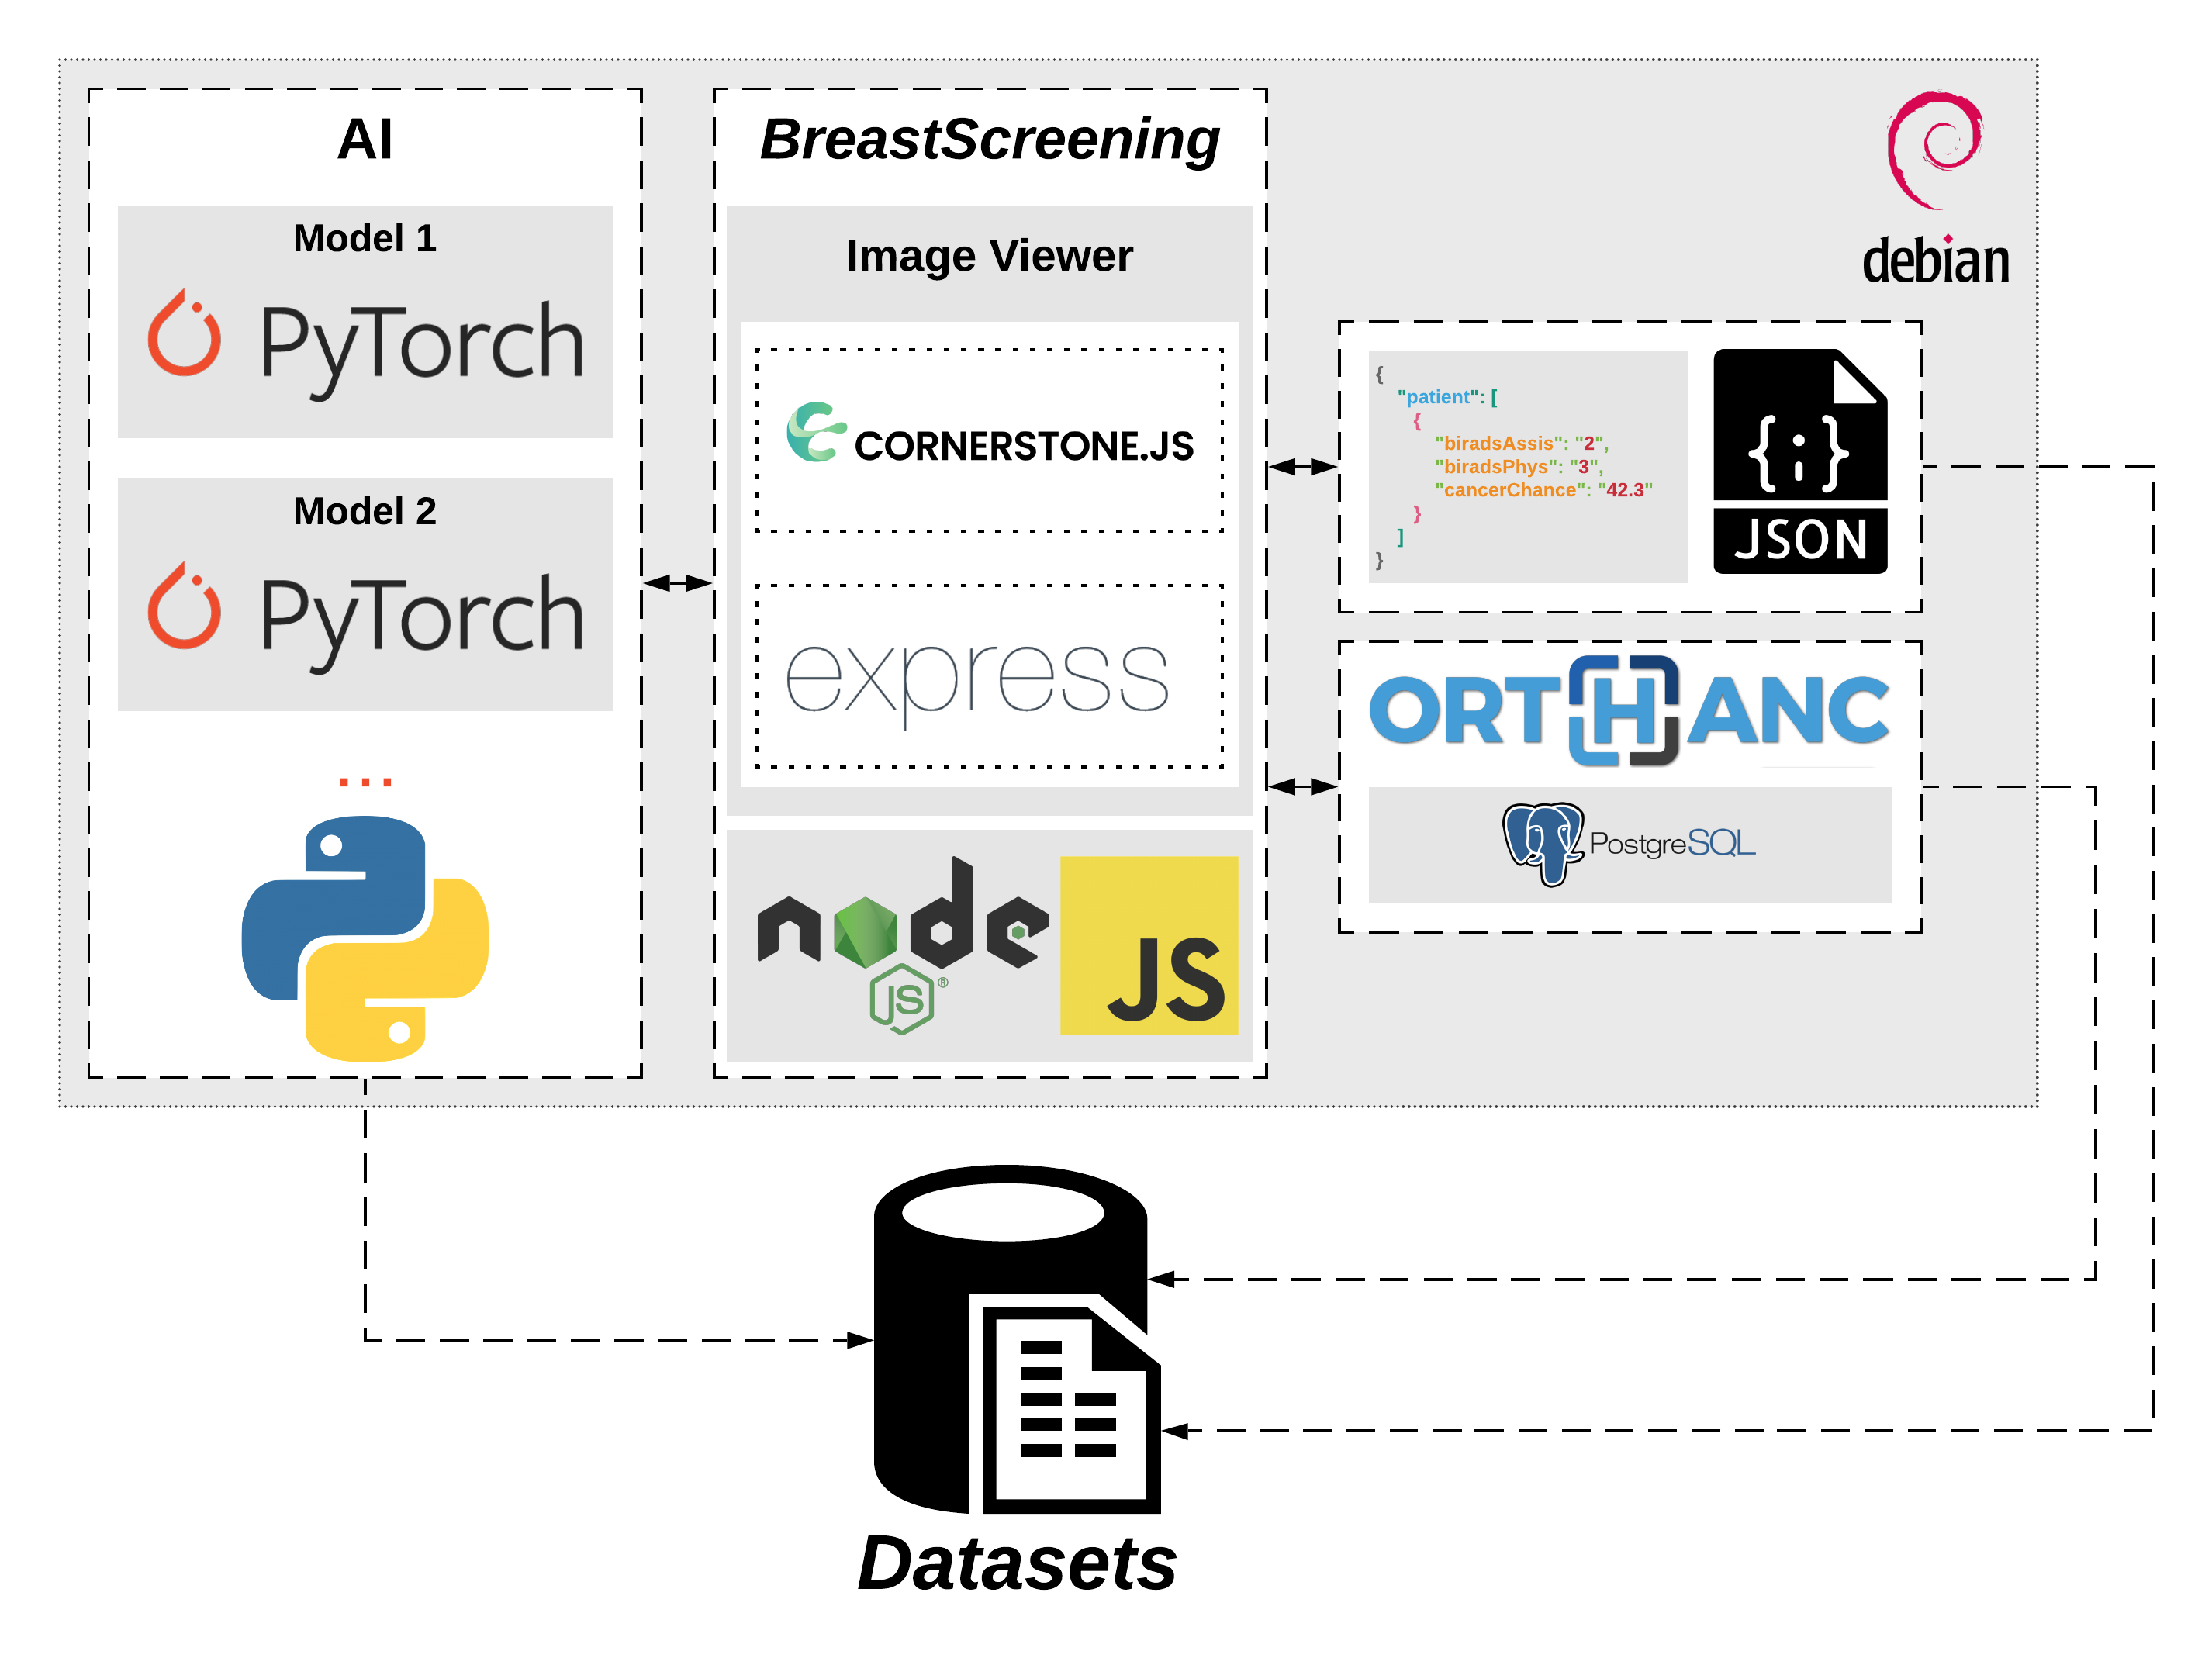
\includegraphics[width=0.80\linewidth]{images/fig041}
\caption{{\it BreastScreening-AI} Architecture: the main components of the system are AI Application, Image Viewer, Datasets and DICOM Storage. The Image Viewer of {\it BreastScreening} framework will provide essential interaction tools for radiologists. A study list is fetched from the Orthanc server, and through CornerstoneJS the radiologist can manipulate the image, interacting with the assistant at the same time.}
\label{fig:fig041}
\end{figure}
%%%%%%%%%%%%%%%%%%%%%%%%%%%%%%%%%%%%%%%%%%%%%%%%%%%

It should be noted that the {\it BreastScreening} core~\cite{10.1145/3399715.3399744} was developed in JavaScript with jQuery\footnotemark[21]~\cite{CALISTO2022102285} for \ac{HTML} document manipulation, event handling of the \ac{UI} interactions, such as mouse events, and with look \& feel improvements.
Additionally, a {\it dicomParser}~\cite{CALISTO2021102607} was used for parsing \ac{DICOM} files.
The \ac{DICOM} files can be loaded by drag-and-drop into the browser window on the Orthanc  (Figure~\ref{fig:fig041}) view.
Loaded images can be further displayed on both views but with different visualization configurations.
After the loading stage, images are automatically arranged according to the scan IDs from the \ac{DICOM} files.

%%%%%%%%%%%%%%%%%%%%%%%%%%%%%%%%%%%%%%%%%%%%%%%%%%%
\footnotetext[21]{\href{https://jquery.com}{jquery.com} - a fast, small, and feature-rich {\it JS} library for the GUI. {\it JQuery} is generic, as it can be configured to render many different types of views.}
%%%%%%%%%%%%%%%%%%%%%%%%%%%%%%%%%%%%%%%%%%%%%%%%%%%

Finally, for this assistant, the DenseNet was developed using \href{https://pytorch.org/}{PyTorch}~\cite{NEURIPS2019_bdbca288}.
More specifically, \href{https://pytorch.org/}{PyTorch} is a \ac{DL} library that is widely used by the \ac{ML} community due to its imperative and ``Pythonic'' programming style.
The library performs immediate execution of dynamic tensor computations with automatic differentiation and \ac{GPU} acceleration, and does so while maintaining performance comparable to the fastest current libraries for \ac{DL} methods.
The availability and normalization of general-purpose massively parallel hardware, such as \acp{GPU}, provided the computing power required to this thesis.
Thus, \href{https://pytorch.org/}{PyTorch} was used under this work  (Figure~\ref{fig:fig041}) to facilitate the implementation of \ac{DL} methods and easily integrate the methods into intelligent agents.

\subsection{Acquired Medical Imaging Datasets}
\label{sec:app003003004}

In order to control the medical imaging information, radiologists interact with in a sub-sequence study.
The {\it BreastScreening-AI} was fixed to operate on a limited subset of 289 classified patients from the collected dataset at \acf{HFF}, an \ac{EPE} institution.
In fact, the acquired dataset of medical images contains more than 200 000 \ac{DICOM} files from a total of 338 patients.
For this work, each of the 289 patients was classified by the head of radiology of Medical Imaging Department at \ac{HFF}.
Then, the head of radiology provided both \ac{BI-RADS} values of the pre-biopsy and pathological results of each patient.

From the pre-biopsy classification, the acquired and curated dataset was divided into three distinct patient types:
{\bf P1} with low severity, {\it i.e.}, BIRADS $\leq$ 1;
{\bf P2} with medium severity, {\it i.e.}, 1 $<$ BIRADS $\leq$ 3; and
{\bf P3} with high severity, {\it i.e.}, BIRADS $>$ 3;
on all possible modalities (\ac{MG}, \ac{US} and \ac{MRI}).
Each radiologist will open each patient ({\it e.g.}, {\bf P1}, {\bf P2} or {\bf P3}), that is chosen randomly, and will examine the set of images.
The dataset resulted from work done by eight of the 45 clinicians.
All the eight clinicians are resident radiologists of \acl{HFF}, working directly with the head of radiology of this institution.

\subsection{Model Description}
\label{sec:app003003005}

A fundamental component in the designed \ac{UI} is the integration of a \ac{DNN} ({\it i.e.}, DenseNet).
A DenseNet is capable of automatically providing the classification for the lesion severity of the exam.
For this study, the DenseNet~\cite{Huang_2017_CVPR} architecture used in {\it BreastScreening-AI} was DenseNet-161.
The DenseNet was initially pre-trained on ImageNet~\cite{10.1145/3351095.3375709}, a large dataset of 1.2 million images from 1,000 classes.
This is an important step, to regularize the network whenever small sets are available for training.
The network parameters were fine-tuned using the acquired and curated medical dataset.
This is accomplished by removing the last layer and replacing it with a new fully-connected layer for five classes, corresponding to the \ac{BI-RADS} (from 1 to 5) values.

To ensure a fair and unbiased evaluation of model performance, the curated dataset was split into two disjoint sets: a training set and a testing set.
The training set was used to fine-tune the weights of the architecture to the medical dataset acquired and curated under this thesis, while the testing set was held out exclusively for evaluation.
It should be noted that in the experimental evaluation, only the test set was used, and radiologists were asked to perform patient diagnosis ({\it i.e.}, {\bf P1}, {\bf P2} or {\bf P3}) to assess the model's diagnostic accuracy.
By using a separate test set, the generalization ability of the model to unseen data can be evaluated, providing more confidence in the model's performance when applied to new datasets.

%%%%%%%%%%%%%%%%%%%%%%%%%%%%%%%%%%%%%%%%%%%%%%%%%%%
\begin{figure}[htbp]
\centering
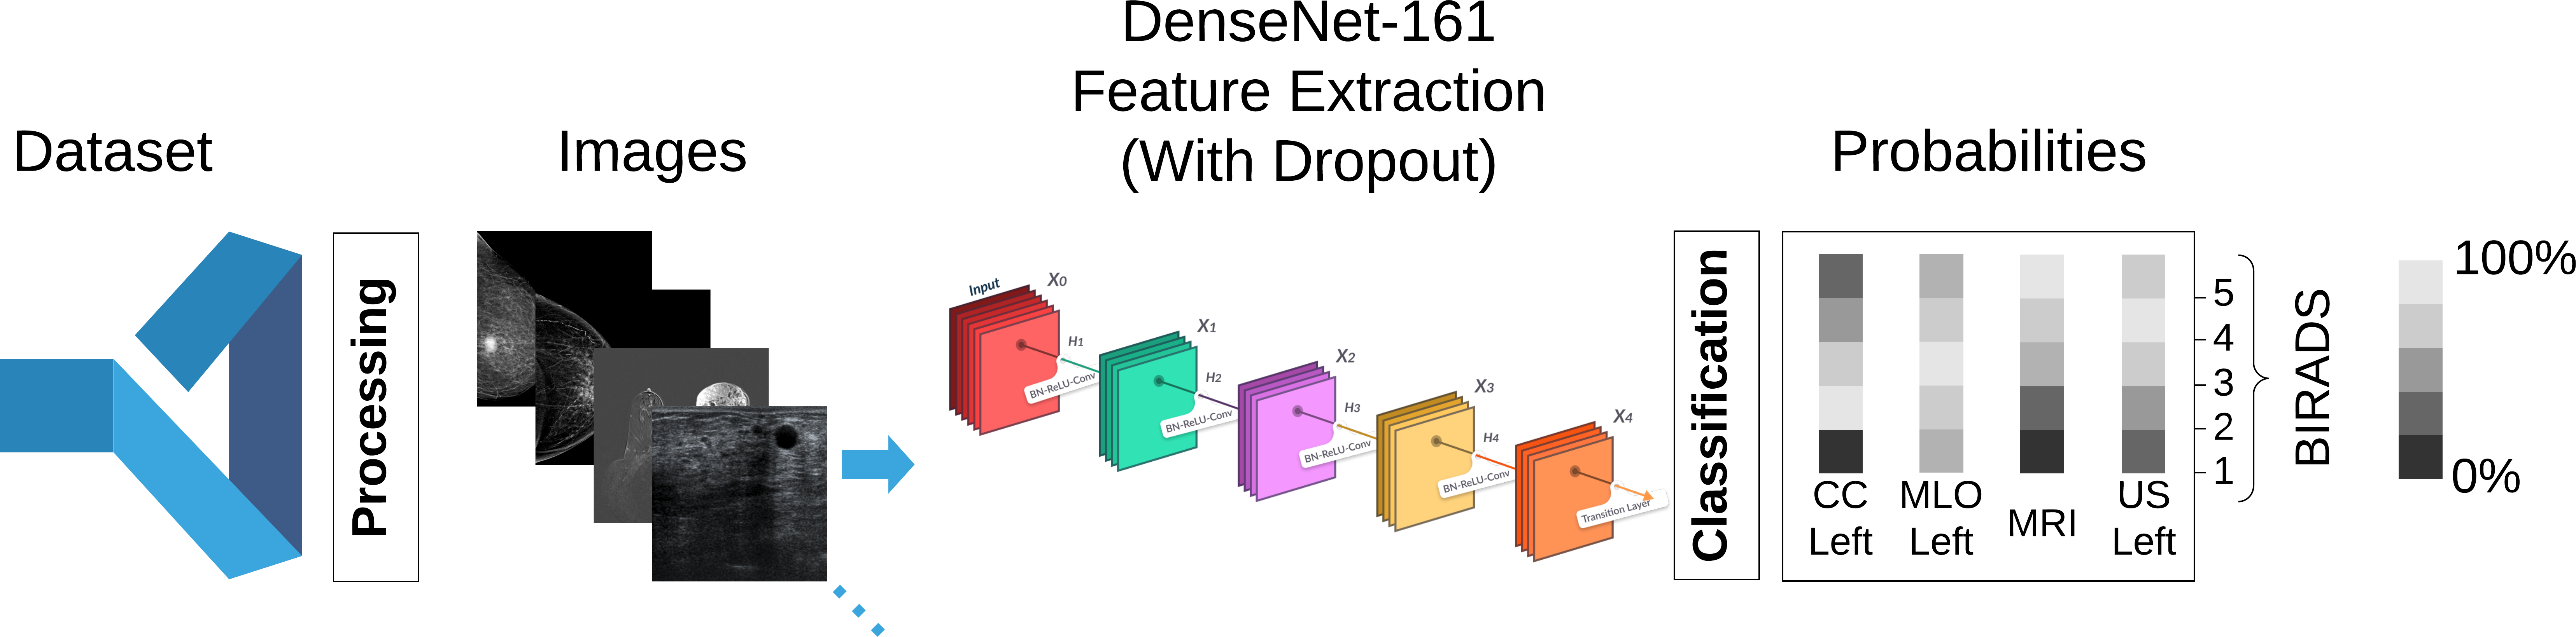
\includegraphics[width=\textwidth]{images/fig042}
\caption{DenseNet extracts features from images using dense blocks to efficiently compute the probability of each class. Classification probabilities are calculated and, in the end, the intelligent agent display the highest probability ({\it i.e.}, from 0\% to 100\%) of all images from that patient. Moreover, the resulted Classification/Probabilities square can also be displayed to provide some kind of XAI to clinicians.}
\label{fig:fig042}
\end{figure}
%%%%%%%%%%%%%%%%%%%%%%%%%%%%%%%%%%%%%%%%%%%%%%%%%%%

In this study, all modalities were evaluated using the same model, which was trained on a curated dataset.
To prepare the dataset for training, a pre-processing step was applied that included resizing the images to $224\times 224$ pixels using bilinear interpolation, as well as normalization to remove the mean and standard deviation.
This pre-processing step is similar to the one used in the ImageNet dataset. The training process utilized the Adam optimizer~\cite{CALISTO2022102285} with the default parameters, including a learning rate of $10^{-3}$ and weight decay of $10^{-4}$.
During training, the model fine-tuned the weights of the architecture to the medical dataset acquired and curated under this study.
In order to evaluate the performance of the model, a hold-out test set was used, which was separated from the curated dataset for fairness purposes.
Only the test set was used for experimental evaluation, and radiologists were asked to perform patient diagnoses on the test set.

To prevent overfitting, online data augmentation was employed using random cropping and random horizontal flipping.
The model was trained using cross-entropy loss, where model predictions after softmax were compared with classifications provided by radiologists.
During testing, unseen images underwent the same pre-processing steps as during training, and the model predictions and classifications were recorded.
The model achieved an accuracy of 94.81\% on the test set using this approach.

\section{Additional Findings \& Analysis}
\label{sec:app003004}

In this section, the section experimentally shows the usefulness of integrating the Human-\ac{AI}, namely its gains when compared to the single radiologist performance.
The experimental evaluation will be conducted to map the \acp{RQ} formulated in Section~\ref{sec:chap005001002} of Chapter~\ref{chap:chap005}.
The study will comprise on the following setups.
The collaboration (within-subject) was distributed into three scenarios: (i) {\it Clinician-Only}; (ii) {\it Clinician-AI}; and (iii) {\it AI-Only}.
However, we are only considering the first two scenarios for this analysis, as the AI-Only is not involving the user.
For each scenario, three patient classes are considered.
Concretely, {\it Low}, {\it Medium} and {\it High} severities.
Each class concerns the lesion severity in the \ac{BI-RADS} score, as ${\rm BIRADS} = 1$, ${\rm BIRADS} \in\{2, 3\}$ and, ${\rm BIRADS}\in\{4, 5\}$, respectively.

\subsection{{\it SUS Scores} vs {\it SUS Positive Questions}}
\label{sec:app003004001}

The generated results of the \ac{SUS} questionnaire are depicted in Figures \ref{fig:fig033} and \ref{fig:fig034}.
On the one hand, Figure ~\ref{fig:fig033} shows the results obtained with
{\it current} (Clinician-Only) scenario.
On the other hand, Figure~\ref{fig:fig034} shows the results with introducing the {\it assistant} (Clinician-AI) scenario.
Both study conditions can be compared to understand usability improvements from the Clinician-Only to Clinician-AI scenarios.
However, this claim will be furthered discussed later (Section~\ref{sec:app003005002}).

In short, the Clinician-Only condition obtained 22\% of agreement against an obtained 69\% for the Clinician-AI condition, revealing a higher acceptance for using the intelligent agent (Figure~\ref{fig:fig034}).
This means that despite clinicians' resistance of change for new tools~\cite{10.1145/3132272.3134111}, clinicians are now accepting this novel intelligent agents to support their clinical workflow.
Another clear fact to explain these values are the results for the easy of use.
In those results, the Clinician-AI condition reveals an 85\% of agreement against the 71\% for the Clinician-Only condition.
Conversely, 82\% of clinicians found that the various functions of the intelligent agent were well integrated with the workflow.
The confidence level with the Clinician-AI condition was also very high, reaching 80\% on this condition.

Values of user confidence are also important to detail.
While using the Clinician-Only condition, clinicians felt confident, where 53\% ``Agree'' and 31\% ``Strongly agree'' with this \ac{SUS} sentence.
A total of 84\% of an agreement under the Clinician-Only condition.
But more important, with the introduction of an intelligent agent this value was improved by far.
Although the total agreement value for the Clinician-AI condition is inferior with 80\% in comparison to the Clinician-Only condition, about 67\% of clinicians ``Strongly agree'' with the \ac{SUS} sentence.
Due to the high improvements of the ``Strongly agree'' sentence, it can be denoted that intelligent agents are increasing high values of confidence.
Such comparison will be further discussed to clarify the achieved results (Section~\ref{sec:app003005002}).
Indeed, values of confidence will be extremely important to understand the impact for the introduction of \ac{AI} systems in the medical workflow, which will also be addressed with values of {\it trust} in Chapter~\ref{chap:chap006}.

%%%%%%%%%%%%%%%%%%%%%%%%%%%%%%%%%%%%%%%%%%%%%%%%%%%
\begin{figure}[htpb]
\centering
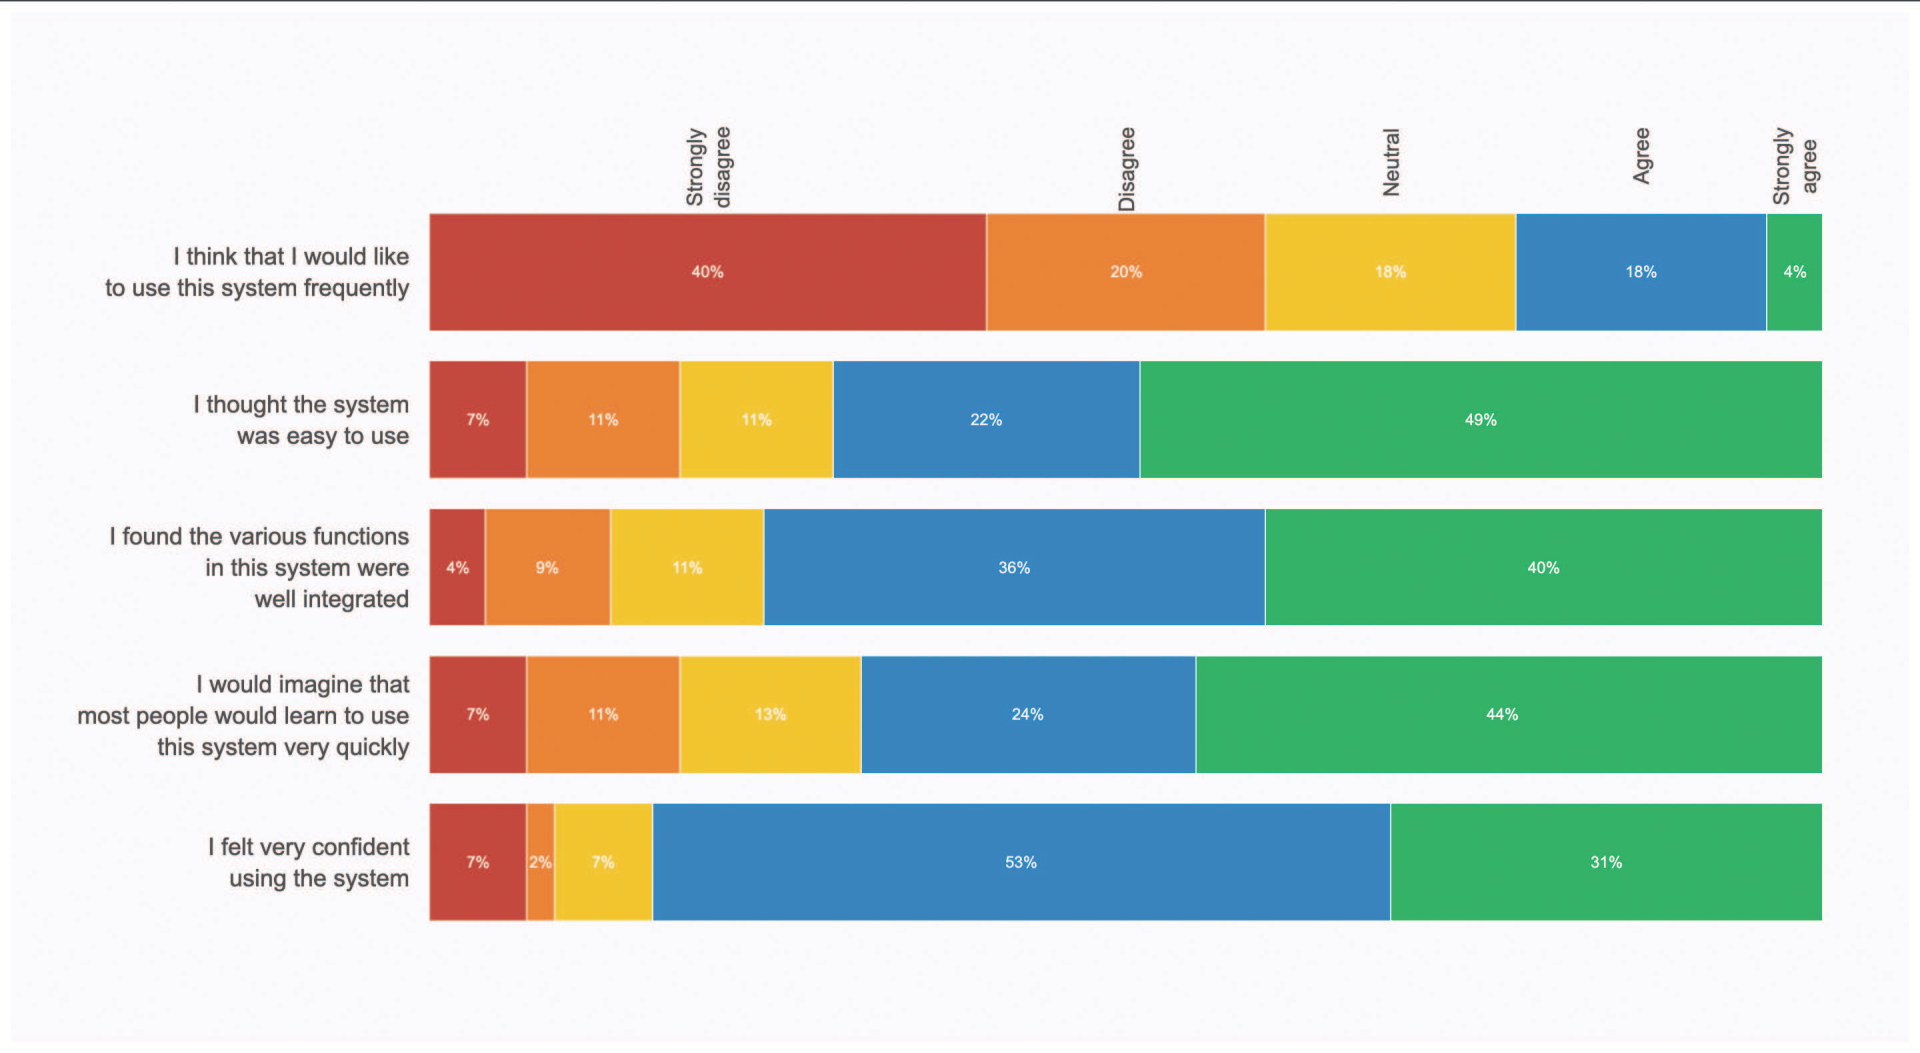
\includegraphics[width=\textwidth]{images/fig033}
\caption{Results of SUS with Positive Questions for the {\it current} (Clinician-Only) scenario. Each color and respective bar number indicate the mean score for the question, {\it i.e.}, ranging from 1 = ``Strongly disagree'' to 5 = ``Strongly agree'' scale. This figure represents the positive questions. The ``Strongly agree'' is the optimal value. From the reported results, a majority of the clinicians agree that the system was easy to use and with well-integrated functionalities.}
\label{fig:fig033}
\end{figure}
%%%%%%%%%%%%%%%%%%%%%%%%%%%%%%%%%%%%%%%%%%%%%%%%%%%

%%%%%%%%%%%%%%%%%%%%%%%%%%%%%%%%%%%%%%%%%%%%%%%%%%%
\begin{figure}[htpb]
\centering
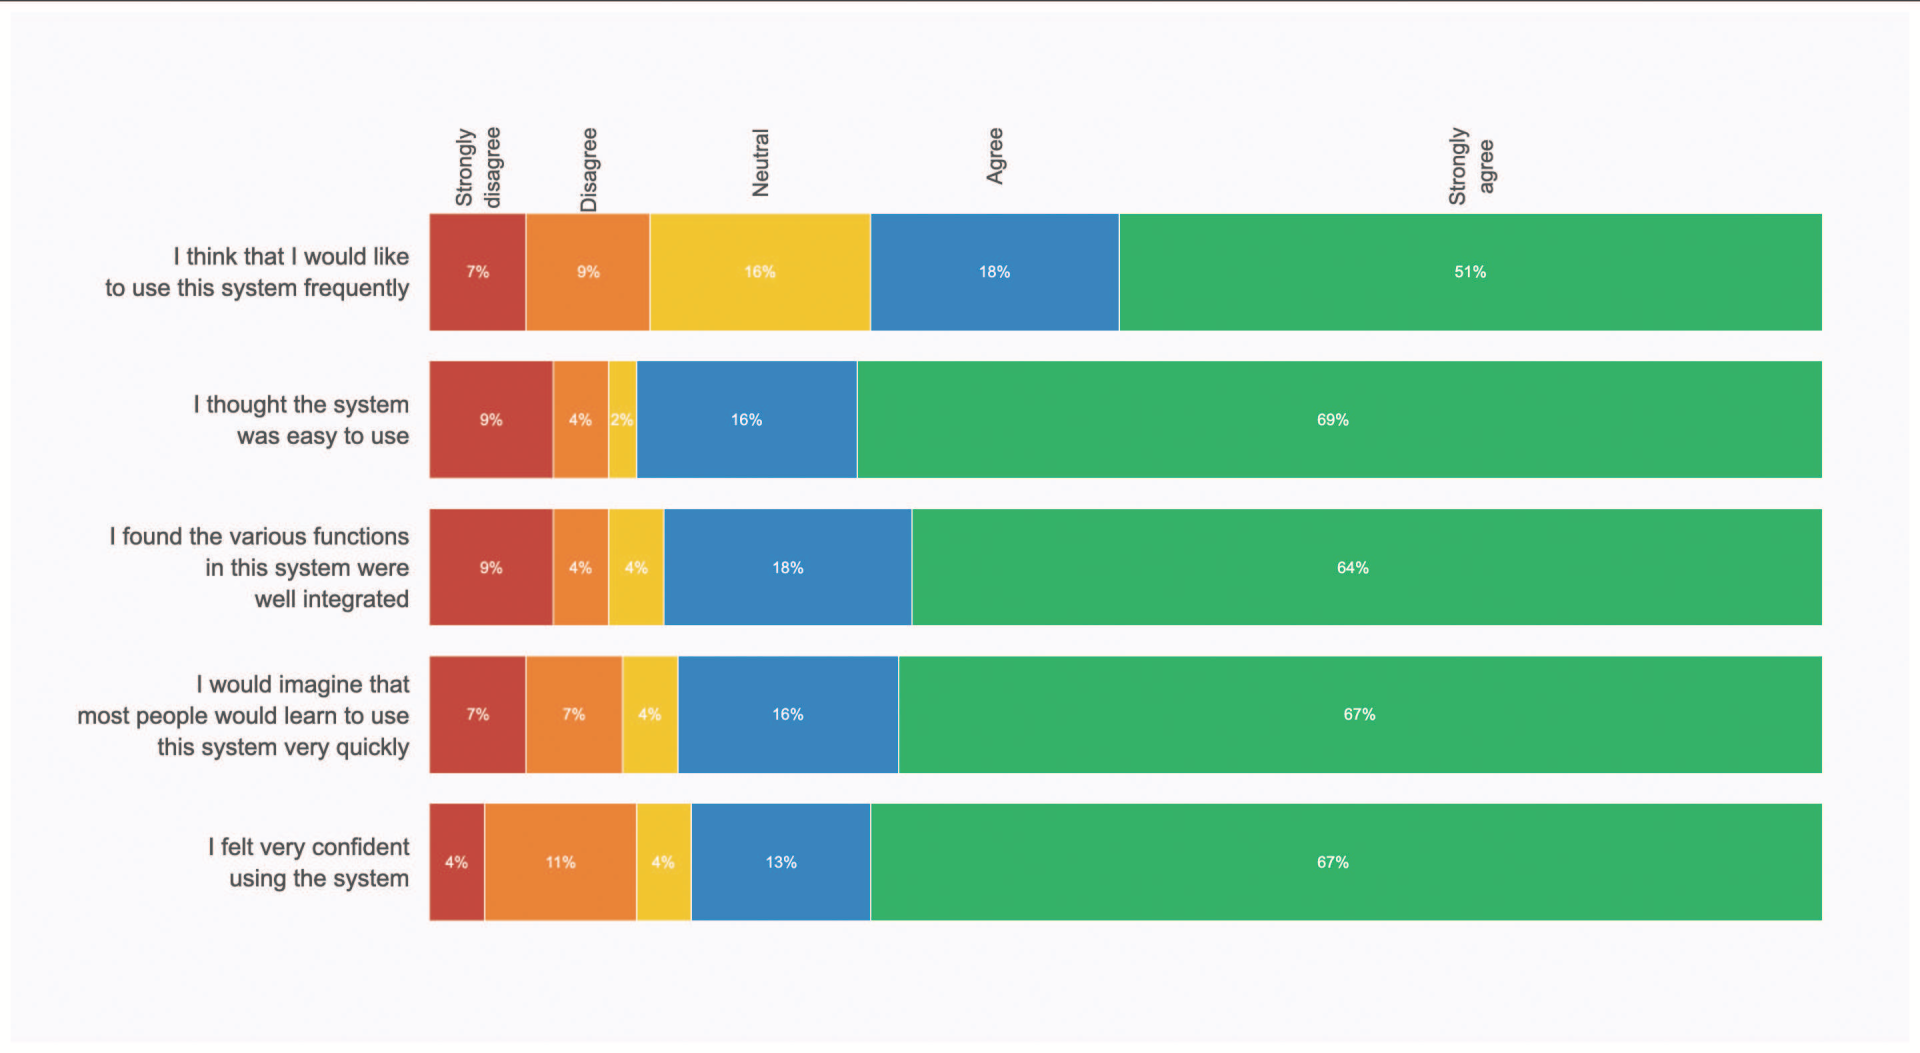
\includegraphics[width=\textwidth]{images/fig034}
\caption{Results of SUS with Positive Questions for the {\it assistant} (Clinician-AI) condition. This Clinician-AI condition was well accepted by clinicians. Almost all clinicians would like to use this system frequently. Moreover, they consider the system much easier to use and with higher integrated functionalities. Last but not least, clinicians learn more quickly and with more confidence this Clinician-AI condition.}
\label{fig:fig034}
\end{figure}
%%%%%%%%%%%%%%%%%%%%%%%%%%%%%%%%%%%%%%%%%%%%%%%%%%%

%%%%%%%%%%%%%%%%%%%%%%%%%%%%%%%%%%%%%%%%%%%%%%%%%%%
\begin{figure}[htbp]
\centering
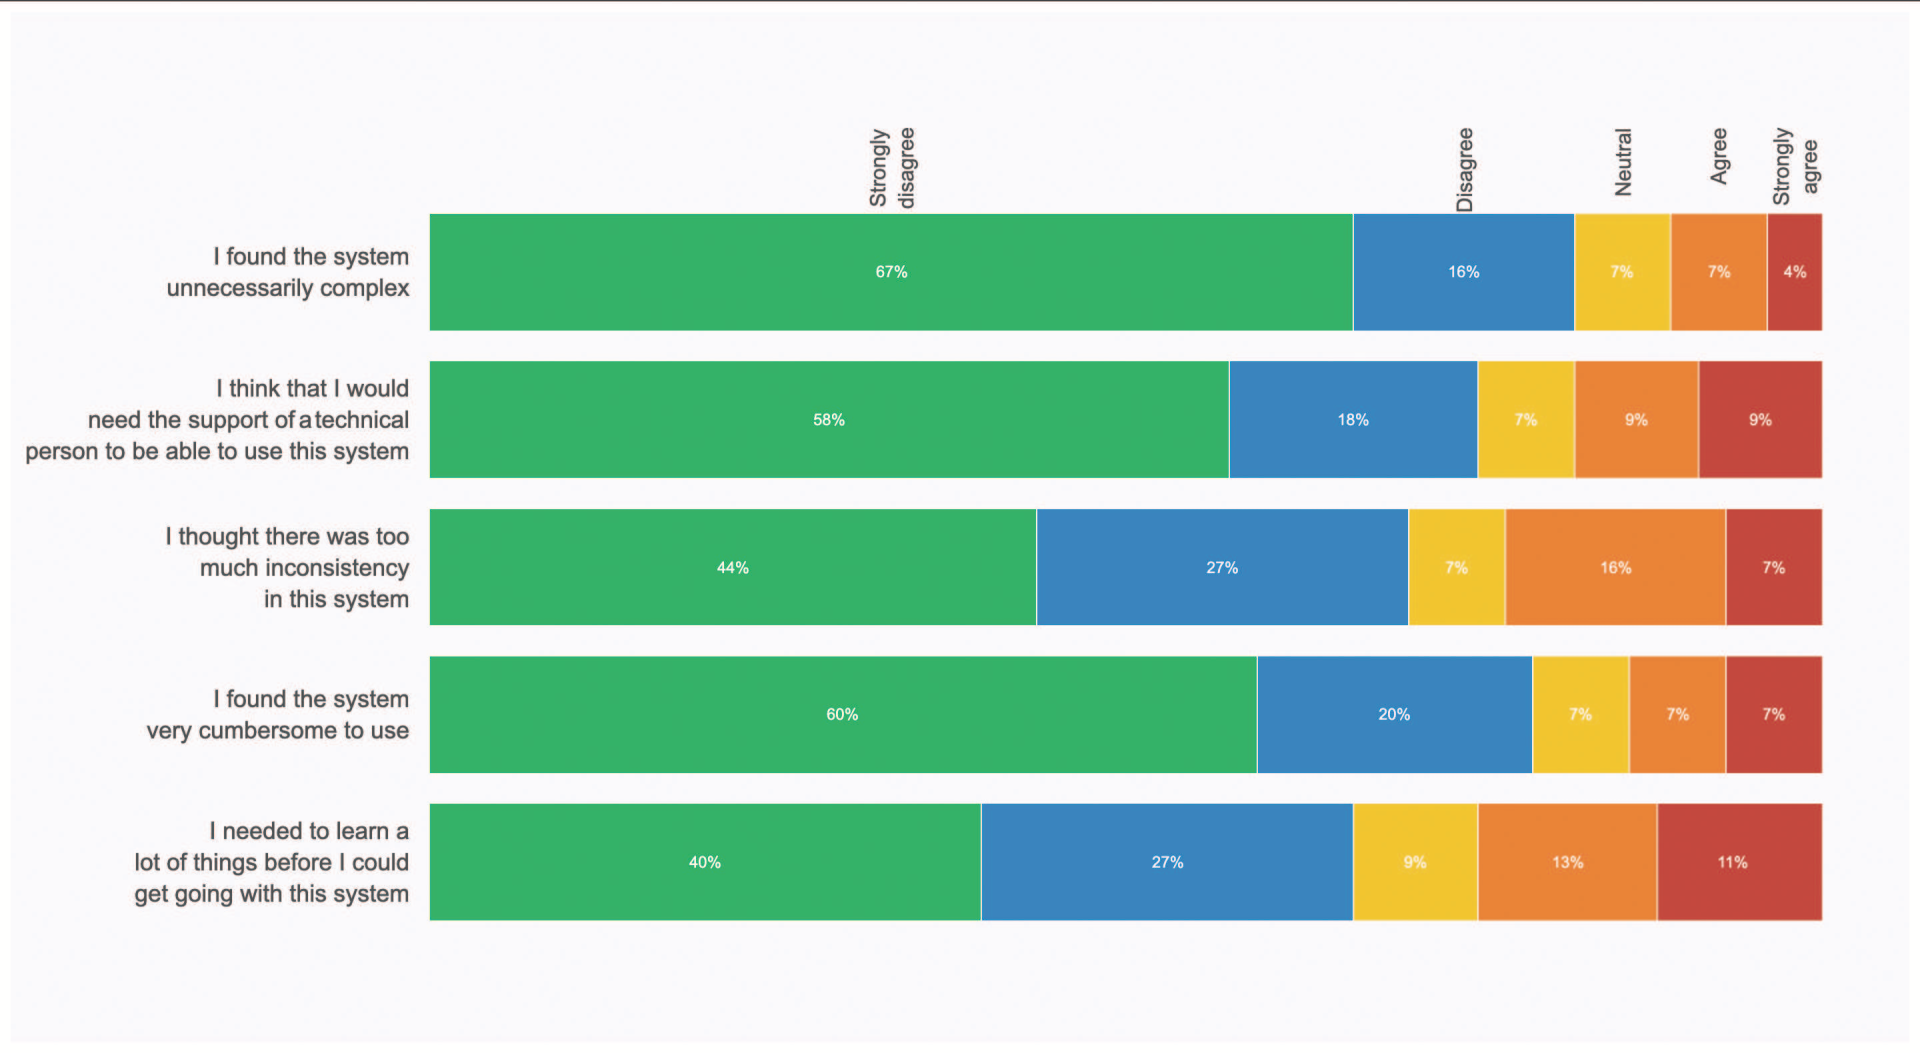
\includegraphics[width=\textwidth]{images/fig035}
\caption{Results of SUS with Negative Questions for the Clinician-Only condition. In this case, it can be observed that 23\% found the system inconsistent and 24\% felt that need to learn before interacting with the system.}
\label{fig:fig035}
\end{figure}
%%%%%%%%%%%%%%%%%%%%%%%%%%%%%%%%%%%%%%%%%%%%%%%%%%%

%%%%%%%%%%%%%%%%%%%%%%%%%%%%%%%%%%%%%%%%%%%%%%%%%%%
\begin{figure}[htbp]
\centering
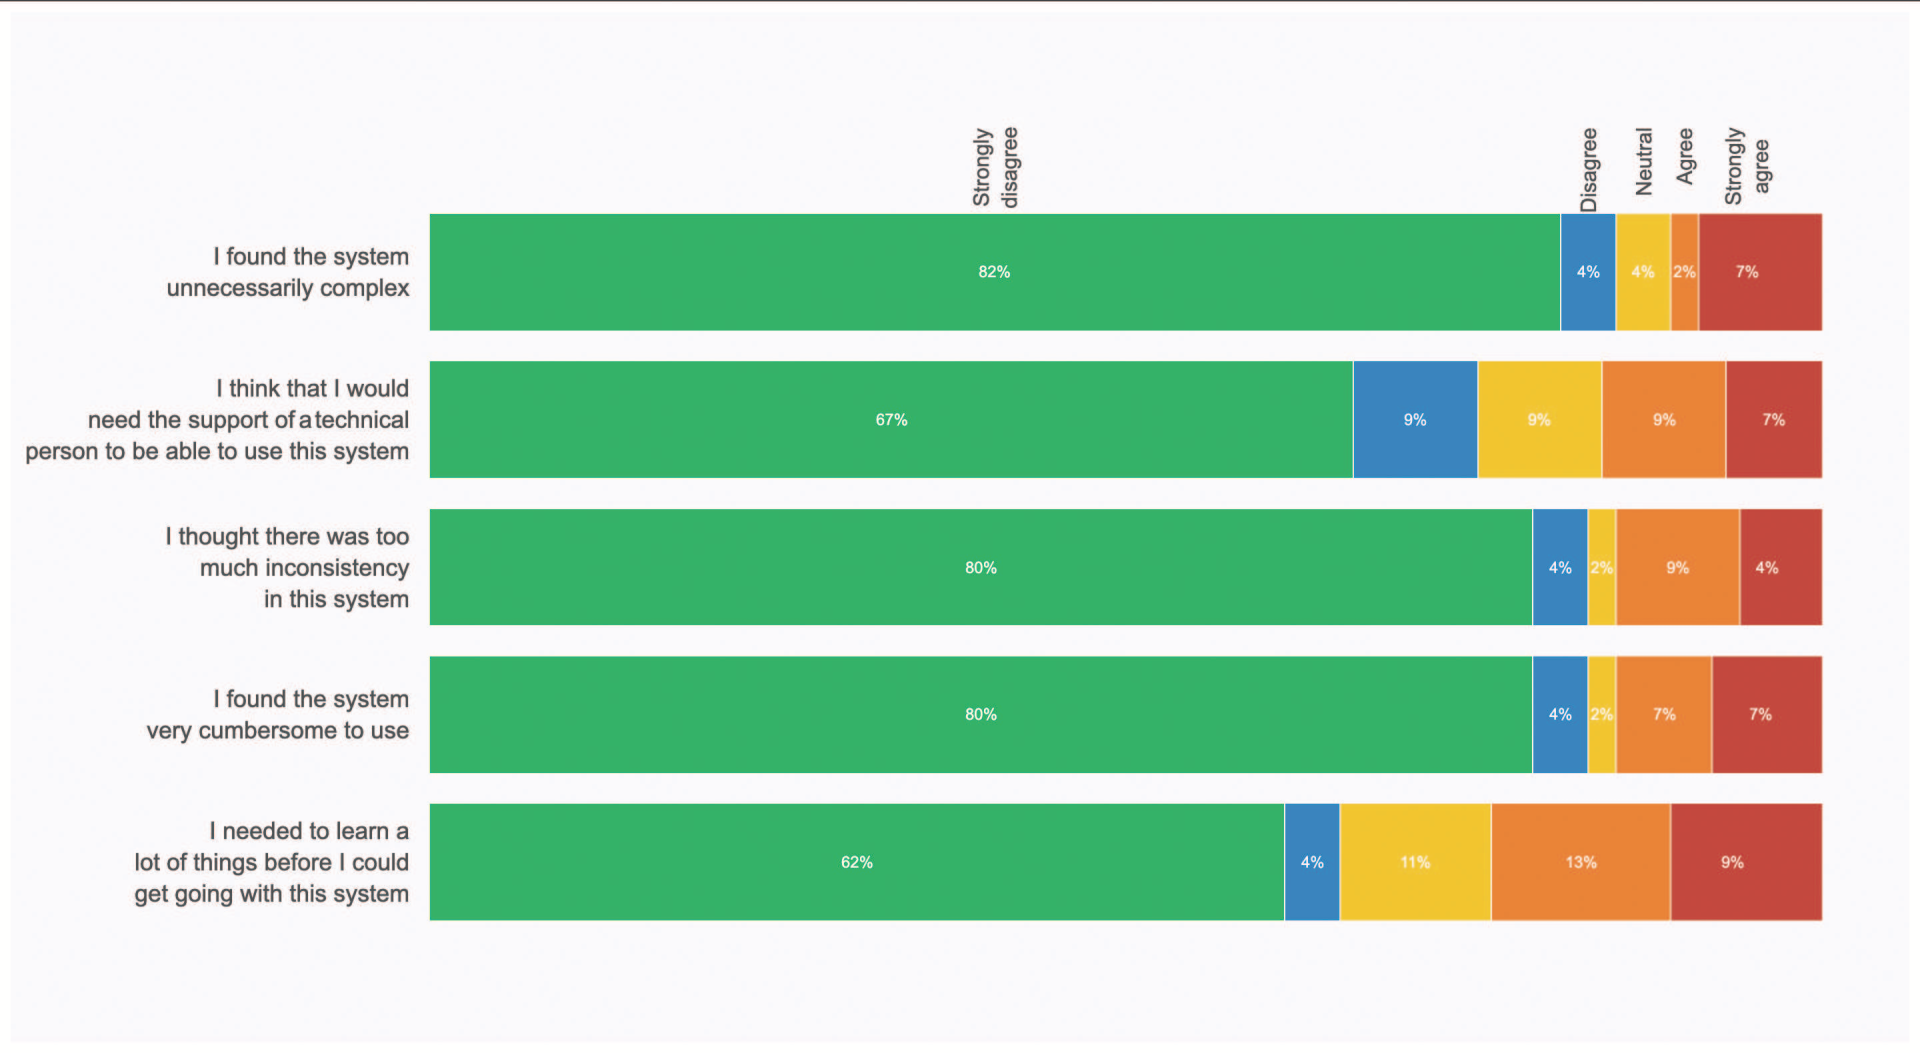
\includegraphics[width=\textwidth]{images/fig036}
\caption{Results of SUS with Negative Questions for the Clinician-AI condition. Comparing the Clinician-AI with the Clinician-Only conditions, it can be observed that clinicians found the Clinician-AI condition less complex, inconsistent and cumbersome.}
\label{fig:fig036}
\end{figure}
%%%%%%%%%%%%%%%%%%%%%%%%%%%%%%%%%%%%%%%%%%%%%%%%%%%

\subsection{{\it SUS Scores} vs {\it SUS Negative Questions}}
\label{sec:app003004002}

Similarly to the previous analysis, here the same study was conducted, but now concerning the negative questions (Figure~\ref{fig:fig036}) of the scale.
Regarding the negative questions (Figure~\ref{fig:fig036}), 86\% of the clinicians disagree that the system is unnecessarily complex.
Suggesting that the introduction of an intelligent agent will not bring more complexity to the diagnostic.
Actually, these results are also paired with the \ac{NASA-TLX} (Tables \ref{tab:tab001} and \ref{tab:tab002}) results to prove this claim.

Concerning both conditions, clinicians also answered two important \ac{SUS} statements addressing system inconsistency and cumbersome.
Specifically, about 44\% of clinicians ``Strongly disagree'' and 27\% ``Disagree'' for system inconsistency statement in the Clinician-Only condition.
On the other hand, about 80\% of clinicians ``Strongly disagree'' and 4\% ``Disagree'' for system inconsistency statement in the Clinician-AI condition.
Thus, by having a total of 84\% of disagreement, the Clinician-AI condition was far improved, against the 71\% of the Clinician-Only, with the introduction of an intelligent agent.
Moreover, in terms of the cumbersome \ac{SUS} statement, about 60\% ``Strongly disagree'' and 20\% ``Disagree'' that the Clinician-Only condition was cumbersome.
For the Clinician-AI condition, 80\% ``Strongly disagree'' and 4\% ``Disagree'' that the system is cumbersome.
A total of 84\% disagreement for cumbersome on the Clinician-AI condition, which is more in comparison to the 80\% of the Clinician-Only.

\subsection{{\it Workload} (Demands)}
\label{sec:app003004003}

The results of the \ac{NASA-TLX} demands, including parameters such as Mental Demand, Physical Demand, and Temporal Demand, are summarized in Table~\ref{tab:tab001}.
For each parameter in the \ac{NASA-TLX}, the data were first normalized, ranked, and then aligned with the \ac{ANOVA}\footnotemark[22] measurements.
The evaluation was conducted under two main conditions, namely the {\it Clinician-Only} condition and the {\it Clinician-AI} condition.
In the following results, we present detailed results from the \ac{NASA-TLX} questionnaire, providing insights into the varying demands under the two conditions.

%%%%%%%%%%%%%%%%%%%%%%%%%%%%%%%%%%%%%%%%%%%%%%%%%%%
\footnotetext[22]{{\it N}: the number of users (Clinicians); $F\textsubscript{var}$: the F-test used for comparing the factors of the total deviation per each variable ({\it var}) categorized by clinical experience; $M\textsubscript{var}$: Mean value of the variable ({\it var}); $SD\textsubscript{var}$: the \acf{SD} per each variable ({\it var}). Notice that from the statistical significance analysis described in Table \ref{tab:tab001} and setting a significance threshold to 0.05, two scenarios are possible to occur. First, if a p-value $>$ 0.05 is obtained, this means that the approaches are not statistically different, better saying. Thus, it can not state anything about the data. On the contrary, if the p-value $<$ 0.05 the approaches are statistically different, since now the value can reject the null hypothesis that states there is not a statistically significant difference between results of the proposed method and the other methods compared.}
%%%%%%%%%%%%%%%%%%%%%%%%%%%%%%%%%%%%%%%%%%%%%%%%%%%

%%%%%%%%%%%%%%%%%%%%%%%%%%%%%%%%%%%%%%%%%%%%%%%%%%%
\begin{table}[htbp]
\begin{tabular*}{\textwidth}{ c @{\extracolsep{\fill}} c c @{\extracolsep{\fill}} c c @{\extracolsep{\fill}} c c }
\toprule
\\
\small
&
\multicolumn{2}{ c }{Mental Demand}
&
\multicolumn{2}{ c }{Physical Demand}
&
\multicolumn{2}{ c }{Temporal Demand}
\\
\cmidrule(lr){2-3}
\cmidrule(lr){4-5}
\cmidrule(lr){6-7}
Condition & F & Sig. & F & Sig. & F & Sig. \\
\\
\bottomrule
\\
Current & 3.392 & 0.027$\star$ & 11.99 & 0.001$\star$ & 10.51 & 0.001$\star$ \\
Assistant & 0.638 & 0.594 & 2.852 & 0.048$\star$ & 0.035 & 0.991 \\
\\
\bottomrule
\hfill
\end{tabular*}
\caption{The ANOVA factorial analysis table regarding NASA-TLX for {\it Mental Demand (MD)}, {\it Physical Demand (PD)} and {\it Temporal Demand (TD)}, where {\it F} is the variation between sample means and the variation within samples. To determine whether any of the differences between the means are statistically significant, the {\it Sig.} was used for significance. On the present study, a 20-point Likert Scale was used regarding Workload. The factorial analysis was described assuming $\alpha = 0.05$. Also, each time $p < 0.05$ it is marked with the $\star$ symbol.}
\label{tab:tab001}
\end{table}
%%%%%%%%%%%%%%%%%%%%%%%%%%%%%%%%%%%%%%%%%%%%%%%%%%%

The \ac{ANOVA} statistical test yields a significant main effect for the Mental Demand (F\textsubscript{Curre.} = 3.39, p\textsubscript{Curre.} = 0.027 $<$ 0.05), Physical Demand (F\textsubscript{Curre.} = 11.99, p\textsubscript{Curre.} = 0.001 $<$ 0.05) and Temporal Demand (F\textsubscript{Curre.} = 10.51, p\textsubscript{Curre.} = 0.001 $<$ 0.05).
On the other hand, the Clinician-AI condition indicates a significant difference only in Physical Demand (F\textsubscript{Assis.} = 2.85, p\textsubscript{Assis.} = 0.048 $<$ 0.05). A detailed comparison is shown in Table~\ref{tab:tab001}.
Despite the higher rates from the \ac{NASA-TLX} over the several Demands (Table~\ref{tab:tab001}), it can be pointed to improvements from the Clinician-Only to the Clinician-AI setup.

From this study, it can be identified that some functionalities contribute significantly to one (or more) types of workloads (criteria variables) in the \ac{NASA-TLX} questionnaire.
For instance, increasing the number of available image modalities on the viewport is strongly associated to Mental Demand.
However, for the Clinician-AI condition it is not possible to take conclusions since the fact that their is no significant main effect.
The overall time duration of manipulating the images ({\it i.e.}, zoom, pan, scroll) is strongly associated to the Physical Demand.
Comparing both Clinician-Only and Clinician-AI conditions, it is possible to be observed a significant main effect and improvements on the Clinician-AI condition.

The time duration of decision-making is strongly associated with Temporal Demand.
Nonetheless, only the Clinician-Only condition follows a significant main effect, making it difficult to do a strong comparison with the Clinician-AI condition.
For simplicity of the results, this work divided the \ac{NASA-TLX} questionnaire items in {\bf Demands} and {\bf Non-Demands} categories.
Next (Section~\ref{sec:app003004004}), the document will report the three items from {\bf Non-Demands} of the \ac{NASA-TLX} questionnaire.

\subsection{{\it Workload} (Non-Demands)}
\label{sec:app003004004}

In evaluating the Non-Demand aspects of the \ac{NASA-TLX}, such as Performance, Effort, and Frustration, we gain valuable insights into user interaction experiences under both Clinician-Only and Clinician-AI conditions.
Notably, significant differences were observed for Performance under the Clinician-Only condition (F\textsubscript{Curre.} = 5.56, p\textsubscript{Curre.} = 0.003 $<$ 0.05), as detailed in Table~\ref{tab:tab002}.
Despite higher rates, improvements were apparent when comparing the Clinician-Only condition to the Clinician-AI condition, suggesting the introduction of an intelligent agent may enhance overall user performance.
However, considering the Effort and Frustration scales is critical, as they provide insights into the mental and emotional toll on the user in both conditions.
High performance at the cost of increased effort or frustration may jeopardize sustainable user engagement.
As such, we must balance these factors optimally to improve \ac{UX}.

%%%%%%%%%%%%%%%%%%%%%%%%%%%%%%%%%%%%%%%%%%%%%%%%%%%
\begin{table}[htbp]
\begin{tabular*}{\textwidth}{ c @{\extracolsep{\fill}} c c @{\extracolsep{\fill}} c c @{\extracolsep{\fill}} c c }
\toprule
\\
\small
&
\multicolumn{2}{ c }{Effort}
&
\multicolumn{2}{ c }{Performance}
&
\multicolumn{2}{ c }{Frustration}
\\
\cmidrule(lr){2-3}
\cmidrule(lr){4-5}
\cmidrule(lr){6-7}
Condition & F & Sig. & F & Sig. & F & Sig. \\
\\
\bottomrule
\\
Current & 0.534 & 0.661 & 5.556 & 0.003$\star$ & 2.392 & 0.082 \\
Assistant & 0.664 & 0.578 & 0.319 & 0.811 & 0.408 & 0.748 \\
\\
\bottomrule
\hfill
\end{tabular*}
\caption{ The ANOVA factorial analysis table regarding NASA-TLX for \textit{Effort (Eff.)}, \textit{Performance (Per.)} and \textit{Frustration (Fru.)}, where {\it F} is the variation between sample means and the variation within samples. To determine whether any of the differences between the means are statistically significant, the {\it Sig.} for significance was used. On the present study, a 20-point Likert Scale was used regarding Workload. The factorial analysis was described assuming $\alpha = 0.05$. Also, each time $p < 0.05$ it is marked with the $\star$ symbol.}
\label{tab:tab002}
\end{table}
%%%%%%%%%%%%%%%%%%%%%%%%%%%%%%%%%%%%%%%%%%%%%%%%%%%

This is a result of the increasing number of visualization modalities, from one in the Clinician-Only condition, to three in the Clinician-AI condition while it is assisted by an \ac{AI} model.
Due to the fact that in Clinician-Only condition, clinicians are analyzing less number of lesions, the effort is less in comparison to the Clinician-AI condition.
For the Clinician-Only condition results, clinicians just diagnosed one modality per each ({\it i.e.}, {\bf P1}, {\bf P2} and {\bf P3}) patient.
On the contrary, for the Clinician-AI results, each clinician diagnoses all the three modalities ({\it i.e.}, \ac{MG}, \ac{US} and \ac{MRI}) per each patient.
In fact, the improvement scores (\textbf{F}) of the proposed Clinician-AI are positive.
Note that, as far as the scores are less than three times the results from the Clinician-Only condition, one can conclude that it is getting better results.

Effort and Frustration do not provide any significant main effect on both Clinician-Only and Clinician-AI conditions.
Therefore, it is not possible to consider any findings regarding these issues.
Nor even the Performance results, since the fact that the {\it assistant} does not represent any significant main effect.
Notwithstanding, these results will be paired (Section~\ref{sec:chap005006}) with the above (Demands) and these (Non-Demands) \ac{NASA-TLX} results with other metrics to discuss the final results with more evidence.

\subsection{{\it Diagnostic Time} vs {\it Breast Severity}}
\label{sec:app003004005}

The results, depicted in Figure \ref{fig:fig037}, detail the total diagnostic time length and breast severity\footnotemark[23] across 289 patients, categorized into three severity groups:
{\bf P1} - Low;
{\bf P2} - Medium; and
{\bf P3} - High.
These insights are critical for assessing system efficiency and accuracy.
Diagnostic time length reflects efficiency and affects patient diagnosis, while accurate breast severity representation denotes severity assessment capability.
User feedback and iterative testing are vital for guiding diagnostic improvements, ensuring the technical proficiency of the \ac{AI} recommendations while addressing the practical needs and preferences of users by taking into account each patient severity group.

%%%%%%%%%%%%%%%%%%%%%%%%%%%%%%%%%%%%%%%%%%%%%%%%%%%
\footnotetext[23]{An available dataset (\href{https://mimbcd-ui.github.io/dataset-uta7-time/}{mimbcd-ui.github.io/dataset-uta7-time}) is provided and made public from the achieved {\it time} data. This will make the work easier to replicate for the scientific community. The link was accessed on the 8th of July, 2023.}
%%%%%%%%%%%%%%%%%%%%%%%%%%%%%%%%%%%%%%%%%%%%%%%%%%%

For the {\bf P1} - Low severity, the Clinician-Only (M\textsubscript{Curre.} = 146, SD\textsubscript{Curre.} = 86.17) was longer than the Clinician-AI (M\textsubscript{Assis.} = 89, SD\textsubscript{Assis.} = 74.13) condition.
However, for the {\bf P2} - Medium severity, the Clinician-Only (M\textsubscript{Curre.} = 78, SD\textsubscript{Curre.} = 48.05) was, again, longer than the Clinician-AI (M\textsubscript{Assis.} = 77, SD\textsubscript{Assis.} = 96.80) condition.
Finally, for the {\bf P3} - High severity, the Clinician-Only (M\textsubscript{Curre.} = 116, SD\textsubscript{Curre.} = 65.70) was longer than the Clinician-AI (M\textsubscript{Assis.} = 64, SD\textsubscript{Assis.} = 86.94) condition.
The \ac{ANOVA} statistical test shows a significant effect over the total {\it Time} for the Clinician-Only (F\textsubscript{Curre.} = 3.25, p\textsubscript{Curre.} = 0.03 $<$ 0.05) condition regarding the clinical experience groups on a {\bf P1} - Low severity case.
Verifying that the introduction of an intelligent agent did not increase the diagnostic time for Low and High severities.

%%%%%%%%%%%%%%%%%%%%%%%%%%%%%%%%%%%%%%%%%%%%%%%%%%%
\begin{figure}[ht]
\centering
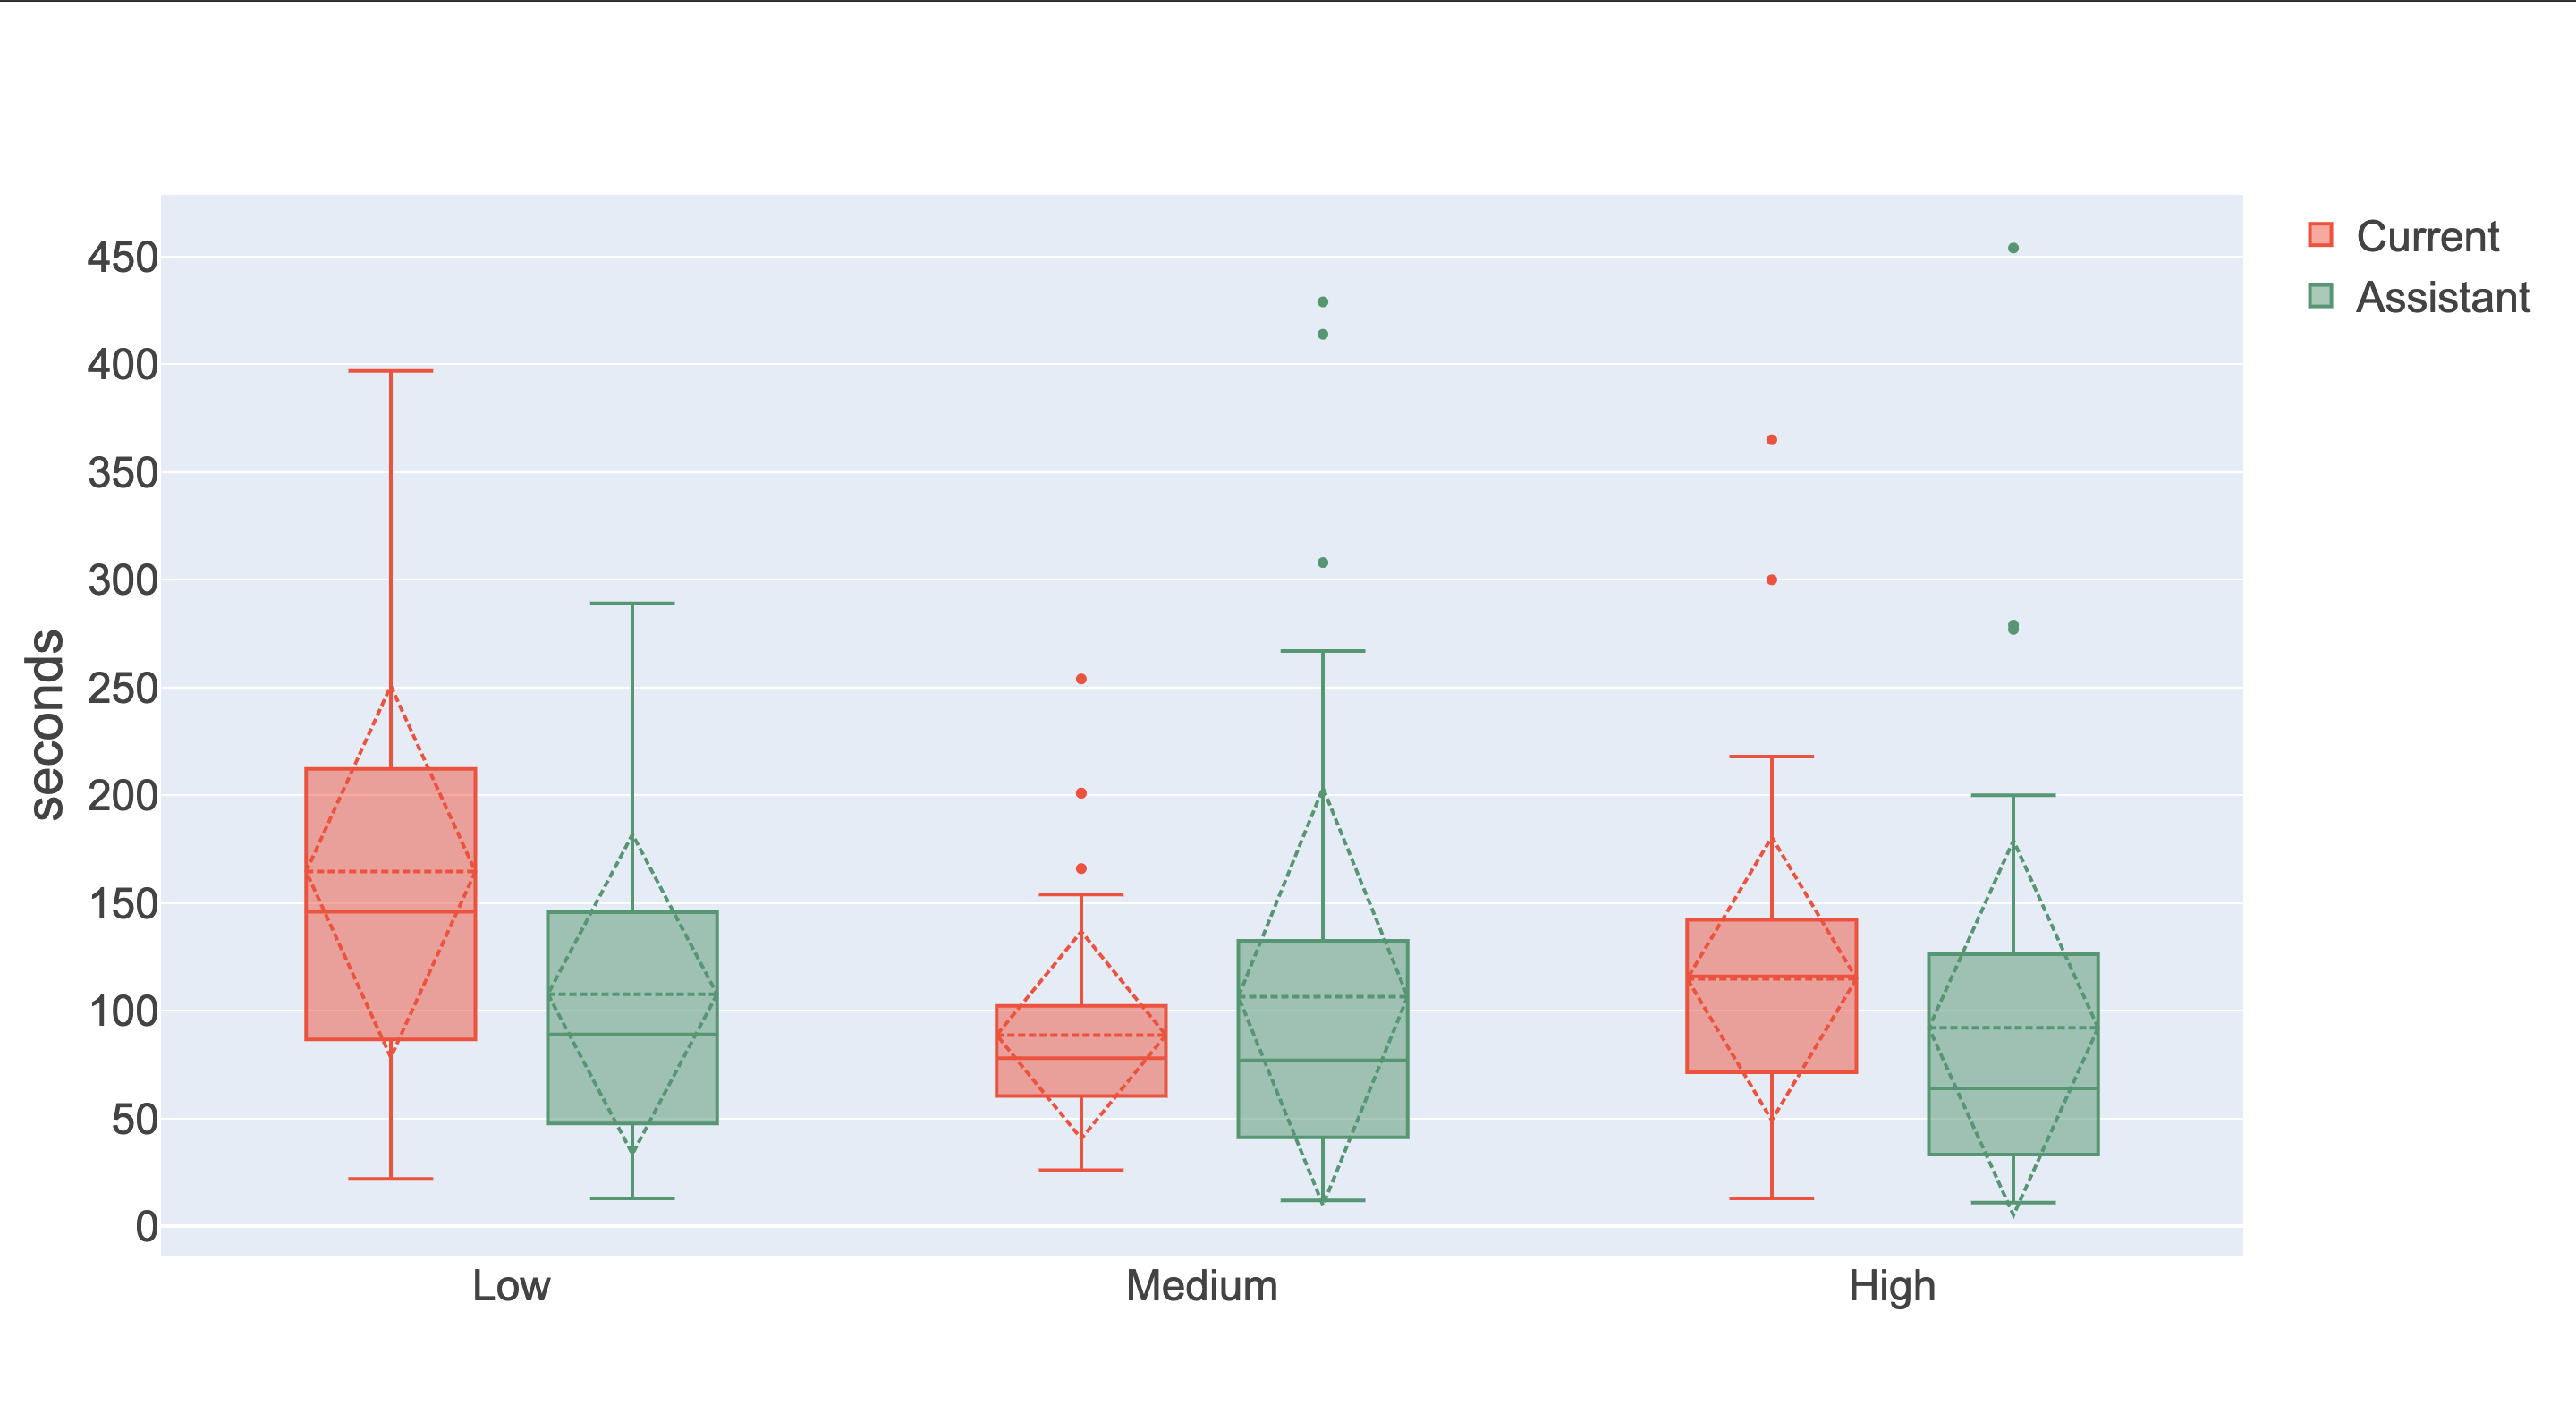
\includegraphics[width=\columnwidth]{images/fig037}
\caption{Relation between diagnostic time length (seconds) and breast severity. Both {\it Current} (Clinician-Only) and {\it Assistant} (Clinician-AI) conditions were compared as Low, Medium and High values of BI-RADS.}
\label{fig:fig037}
\end{figure}
%%%%%%%%%%%%%%%%%%%%%%%%%%%%%%%%%%%%%%%%%%%%%%%%%%%

Planned post-hoc testing~\cite{10.1145/2858036.2858360}, using Tukey's HSD Post-Hoc Comparison (p\textsubscript{Curre.} $<$ 0.05), revealed that for the groups of {\it Juniors}, it significantly increased the time performance and severity accuracy compared to {\it Interns}.
Therefore, the proposed intelligent agent, not only improves time performance (Figure~\ref{fig:fig037}) and diagnostic accuracy (Figure~\ref{fig:fig038}) among the other clinicians' categories of medical experience, but also provides essential support for {\it Interns}.

Although the diagnostic time increased on medium severities, the increase was just residual and will be further discussed (Section~\ref{sec:chap005007}).
These results are answering to what is the workflow impact of intelligent agents for avoiding different types of diagnostics.
Therefore, suggesting that the proposed {\it BreastScreening-AI} tool could positively impact the clinical workflow.
While improving time performance (Section~\ref{sec:app003004009}) and diagnostic accuracy (Section~\ref{sec:app003004009003}), the system is also mitigating the different types of errors in clinical perception.

\subsection{Clinical Impact}
\label{sec:app003004006}

Concerning the assumption that accuracy impacts perceived \ac{UX} of clinicians and acceptance of \ac{AI} systems, Figure~\ref{fig:fig044} and Figure~\ref{fig:fig043} show the metric statistics using the confusion matrix (with 45 clinicians).
More precisely, the performance accuracy can be observed with the proposed \ac{AI} integration (Figure~\ref{fig:fig043}) is superior in comparison with the performance without integration (Figure~\ref{fig:fig044}).
In this confusion matrix, the diagonal shape of the matrix is denoted as being more evident with the introduction of the \ac{AI} (Figure~\ref{fig:fig043}).
Moreover, the diagnostic accuracy is also higher (Table~\ref{tab:tab005}) when the assistant is integrated in the \ac{UI}.
The mean and standard deviation\footnotemark[24] were obtained for the {\it Precision} (M = 0.656, SD = 0.34) and {\it Recall} (M = 0.622, SD = 0.27), respectively, with a 57.69\% of improvement in the F1-score.

%%%%%%%%%%%%%%%%%%%%%%%%%%%%%%%%%%%%%%%%%%%%%%%%%%%
\footnotetext[24]{{\it N}: the number of users (Clinicians); $F\textsubscript{var}$: the F-test used for comparing the factors of the total deviation per each variable ({\it var}) categorized by clinical experience; $M\textsubscript{var}$: Mean value of the variable ({\it var}); $SD\textsubscript{var}$: the \acf{SD} per each variable ({\it var}) denoted in this description of the results.}
%%%%%%%%%%%%%%%%%%%%%%%%%%%%%%%%%%%%%%%%%%%%%%%%%%%

%%%%%%%%%%%%%%%%%%%%%%%%%%%%%%%%%%%%%%%%%%%%%%%%%%%
\begin{table}[htbp]
\centering
\begin{tabular}{|c|c|c|c|c|c|c|}
\hline
\multirow{2}{*}{BIRADS} & \multicolumn{2}{c|}{Precision} & \multicolumn{2}{c|}{Recall} & \multicolumn{2}{c|}{F1-score}   \\ \cline{2-7} 
                        & Clini.-On.      & Clini.-AI    & Clini.-On.     & Clini.-AI    & Clini.-On.     & Clini.-AI    \\ \hline
1                       & 0.01            & 0.69         & 0.76           & 0.91         & 0.02           & 0.78         \\ \hline
2                       & 0.13            & 0.86         & 0.91           & 0.91         & 0.23           & 0.88         \\ \hline
3                       & 0.20            & 0.50         & 0.50           & 0.20         & 0.29           & 0.29         \\ \hline
4                       & 0.20            & 0.99         & 0.61           & 0.68         & 0.30           & 0.81         \\ \hline
5                       & 0.99            & 0.99         & 0.57           & 0.86         & 0.72           & 0.92         \\ \hline
\end{tabular}
\caption{Reported performance of Clinician-Only (Clini.-On.) and Clinician-AI (Clini.-AI) collaborations. The {\it Precision} is the fraction of relevant instances among the classified instances. On the other hand, the {\it Recall} (sensitivity) is the fraction of relevant instances classified over the total amount of relevant instances. The {\it F1-score} is the harmonic mean of precision and recall, giving a balanced measure of precision and recall performance.}
\label{tab:tab005}
\end{table}
%%%%%%%%%%%%%%%%%%%%%%%%%%%%%%%%%%%%%%%%%%%%%%%%%%%

From the \ac{DOTS}\footnotemark[25] questionnaire, 98\% of the 45 clinicians answered that they do understand what the system is thinking.
Also, 93\% of the clinicians trust the system's capability, sustaining our claim regarding the acceptance of the system.
By measuring the accuracy of Clinician-Only and Clinician-AI conditions paired to measurements of trust through the \ac{DOTS} questionnaire, it was possible to answer our claim on {\it what is the impact of precision and recall in clinicians' perceptions} of accuracy and acceptance for the introduction of \ac{AI} systems into their medical workflow.
We concluded that in the context of breast cancer detection and diagnosis, the trade-off between precision and recall is a crucial factor to be considered when implementing \ac{AI} in medical imaging.

%%%%%%%%%%%%%%%%%%%%%%%%%%%%%%%%%%%%%%%%%%%%%%%%%%%
\footnotetext[25]{The DOTS is a 3-item Likert scale questionnaire. In this study, the three questions are scored between 0 and 20.}
%%%%%%%%%%%%%%%%%%%%%%%%%%%%%%%%%%%%%%%%%%%%%%%%%%%

High precision means that a \ac{DL} model returned substantially more relevant results than irrelevant ones.
In Table~\ref{tab:tab005}, we could observe a higher number of \acp{FP} in \ac{BI-RADS} = 1, 2, and 4 between the two conditions.
However, precision alone does not tell us about the ability of the \ac{DL} model to identify all actual positives in the dataset.
In breast cancer detection, \acp{FP} can lead to unnecessary additional testing, anxiety, and distress for the patient.
Yet, compared to \acp{FN}, \acp{FP} are generally considered less harmful, as they can be corrected with further testing and do not result in missed treatment opportunities.

%%%%%%%%%%%%%%%%%%%%%%%%%%%%%%%%%%%%%%%%%%%%%%%%%%%
\begin{figure}[htbp]
\centering
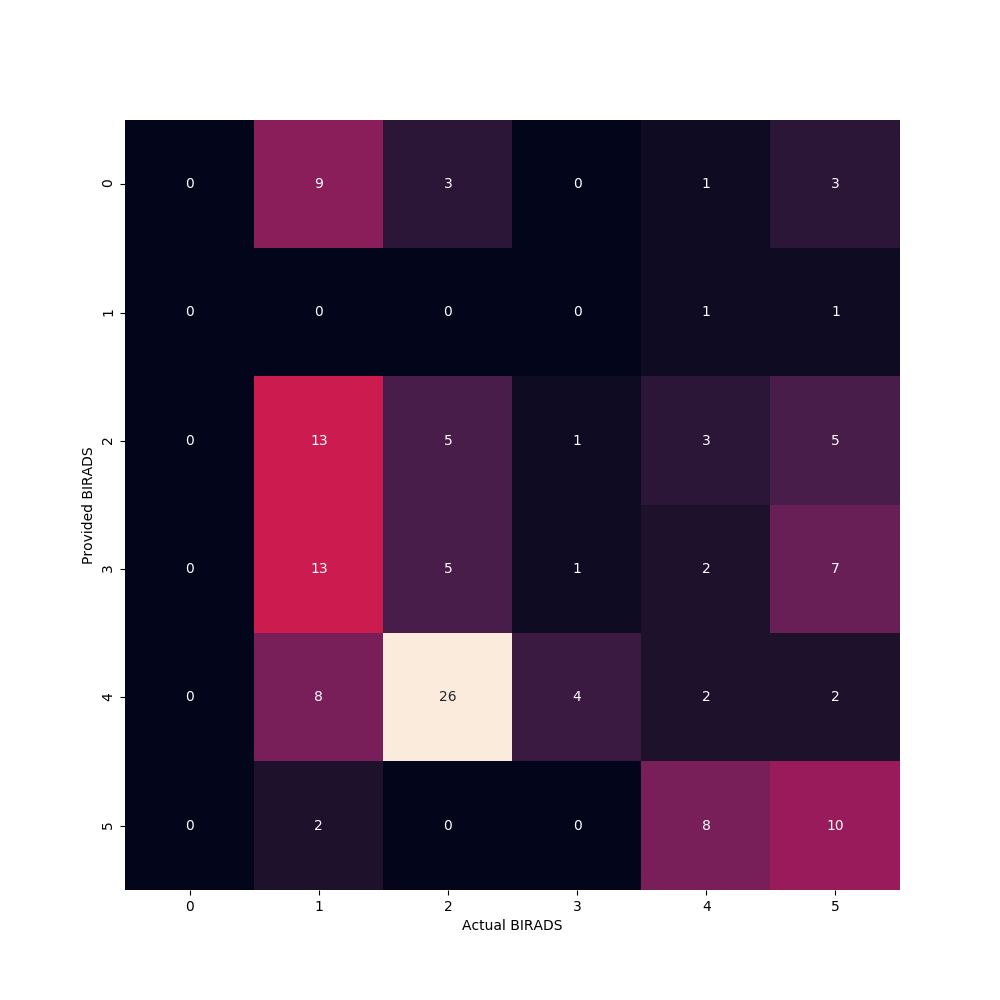
\includegraphics[width=\textwidth]{images/fig044}
\caption{Confusion Matrix without the AI ({\it Clinician-Only}) technique. For this case, the DenseNet results were not used. Each physician directly provided the BI-RADS to the system with no support of AI techniques. The classification accuracy was just 13\% for the number of True-Positives. On the other hand, the number of False-Negatives was 59\% and the number of False-Positives was 28\%. The {\it Provided} value was most accurate in classifying high (BIRADS $\ge$ 4) severity cases. The columns represent the {\it Actual} (biopsy confirmed) category of the objects and the rows represent the {\it Provided} (only physician) value.}
\label{fig:fig044}
\end{figure}
%%%%%%%%%%%%%%%%%%%%%%%%%%%%%%%%%%%%%%%%%%%%%%%%%%%

%%%%%%%%%%%%%%%%%%%%%%%%%%%%%%%%%%%%%%%%%%%%%%%%%%%
\begin{figure}[htbp]
\centering
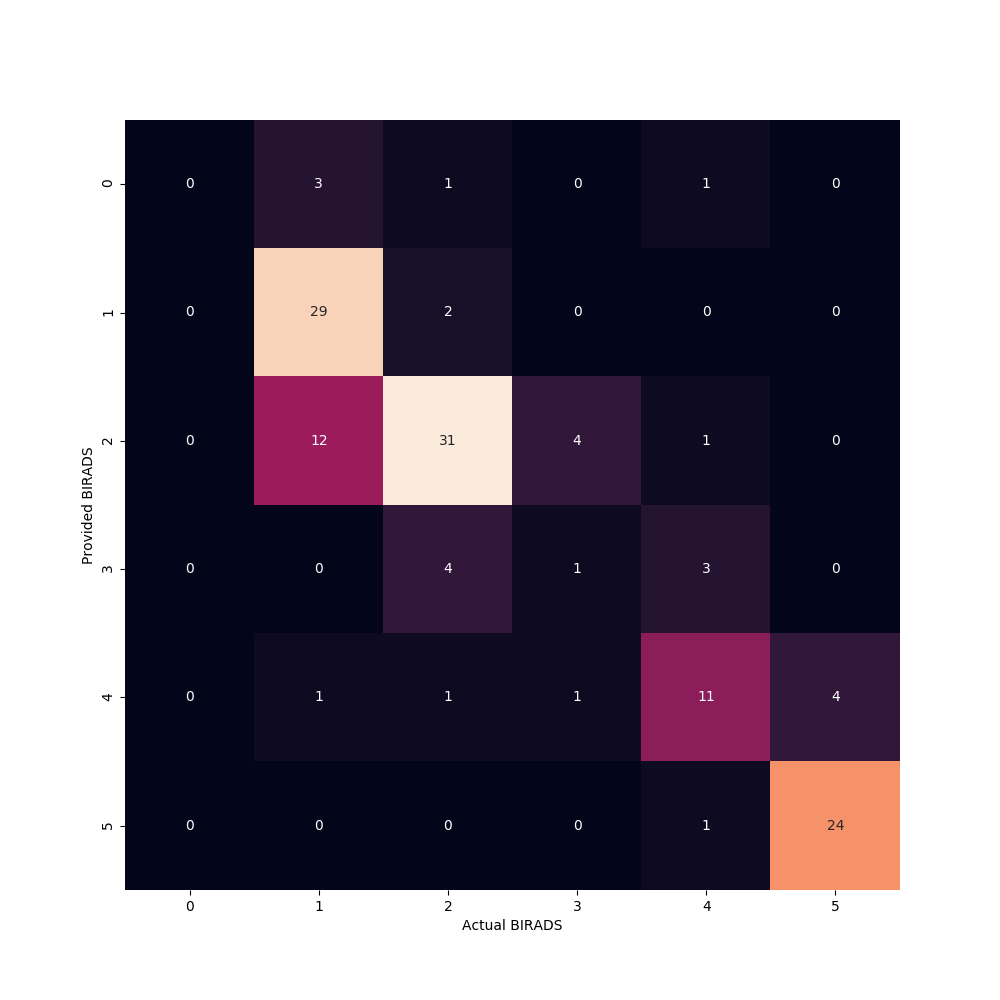
\includegraphics[width=\textwidth]{images/fig043}
\caption{Confusion Matrix with information of the collaboration ({\it Provided}) between physicians and the proposed AI ({\it Clinician-AI}) technique. For this case, a DenseNet results were used among the BI-RADS outputs to support the physician decision. The classification accuracy was 71\% for the number of True-Positives. On the other hand, the number of False-Negatives was 15\% and the number of False-Positives was 14\%, only. The {\it Provided} value was most accurate in classifying low (BIRADS $<$ 2) and high (BIRADS $\ge$ 4) severity cases. The columns represent the {\it Actual} (biopsy confirmed) category of the objects and the rows represent the {\it Provided} (collaboration between physician and AI).}
\label{fig:fig043}
\end{figure}
%%%%%%%%%%%%%%%%%%%%%%%%%%%%%%%%%%%%%%%%%%%%%%%%%%%

On the other hand, high recall means that the \ac{DL} model returned most of the relevant results.
In cases where it fails and produce more \acp{FN}, such as for \ac{BI-RADS} = 3 (Table~\ref{tab:tab005}), we must take into account the small generalizability power of the \ac{DL} model across the dataset (Section~\ref{sec:app004003002} of Appendix~\ref{chap:app004}).
But again, recall alone does not consider the number of irrelevant results that were also returned.
During breast cancer detection, \acp{FN} ({\it i.e.}, when the \ac{AI} system fails to detect cancer that is actually present) can have severe implications.
In our results, these include a 30\% more delayed treatment, progression of the disease, or potentially fatal outcomes for patient cases with \ac{GT} of \ac{BI-RADS} = 3.
Enough to reduce clinicians' overall trust in the \ac{AI} system.
Therefore, maintaining high recall is crucial to ensure acceptance of the \ac{AI} system, since it will correctly identify as many positive cases as possible.

Finally, while the focus is on enhancing recall, efforts should still be made to improve precision as much as possible to minimize the potential harm of \acp{FP}.
Therefore, continual evaluation and refinement of the \ac{AI} system based on feedback from clinicians and outcomes data will be necessary.

\subsection{User Expectations}
\label{sec:app003004007}

Concerning clinicians' needs for explanations (\acs{XAI}), a visual information strategy was adopted that relies on the use of {\it heatmaps} (Figure~\ref{fig:fig032} on Section~\ref{sec:chap005004002002} of Chapter~\ref{chap:chap005}).
Our work takes into consideration the following two functionalities for the colored-visualization:
(1) the lesion circularity or distribution; and
(2) the associated \ac{BI-RADS} value.
It is known that mass morphology is a relevant feature for lesion classification~\cite{maicas2018training}.
The more irregular the lesion is, the more severe its classification will be.
Thus, hot colors are associated with more irregular morphology, improving the user's expectation regarding the final result of the \ac{DL} model.
Concerning the \ac{BI-RADS}, we also assign hot colors for increasing values of the \ac{BI-RADS}. 
This can be easily accomplished by pressing the {\it Explain} ({\it Re-6.2.}) button.

From the \ac{DOTS} questionnaire, the following scores for {\bf Understanding} were obtained.
Concretely, when clinicians {\it press} (M = 19.7, SD = 2.92) or {\it do not press} (M = 10, SD = 7) the  {\it Explain} button, respectively.
Furthermore, the values of trust in the assistant were also much higher (M = 18.81, SD = 2.96) than those of clinicians who did not press the {\it Explain} ({\it Re-6.2.}) button (M = 12.43, SD = 3.21).
Similarly, no significant imbalance was present in prior frequency for using {\it BreastScreening-AI}.
That said, these results support our claim on {\it how do precision and recall affect clinicians' receptiveness and expectations}, changing their capability perceptions on what the \ac{AI} system can do.

Explanations significantly increase clinicians’ perceived level, both in terms of understanding and trust capability.
This implies that designing an intelligent agent can enhance user perception and improve clinician acceptance by providing control over the suggested final diagnostic.
This can be accomplished by assigning to the {\it control} with {\it Accept} or {\it Reject} functionalities as a way to provide (or inhibit) a second opinion, resulted by the assistant.
From \ac{DOTS}, the answers to this questionnaire obtained 76\% of the clinicians that agreed to {\it Accept} with positive benevolence statistics (M = 14.67, SD = 5.24).

In this work, promoting clinicians' management of the final result, revealed a significant (p $<$ 0.05) positive impact, with a higher feeling of control for clinicians that agree with the benevolence of the assistance than for those that did not agree.
Now analyzing the 14\% of clinicians who rejected the \ac{AI} recommendations, it should be highlighted that from those, 52\% of clinicians failed (M = 3.72, SD = 4.68) in the classification, contributing to the higher \acp{FP} or \acp{FN} rates.
This means that they wrongly rejected the suggestion, while the \ac{DL} model was correct for the final diagnostic.

Finally, it was found that the integration of the intelligent agent helps clinicians to improve the final rates, {\it i.e.}, \acp{FP} and \acp{FN}, as well as time performance.
This is related to the number of correctly identified cases during the classification (Figure~\ref{fig:fig043} and Figure~\ref{fig:fig044}) that is always higher than the ones obtained without assistance.
Specifically, the mean values were obtained, with (M = 19.2, SD = 12.81) and without (M = 3.6, SD = 4.03) assistance, respectively.
The values are taken from the diagonal of the confusion matrices.
Furthermore, in terms of time performance, it can be denoted that with the {\it Clinician-AI} (M = 76.67 seconds, SD = 85.96 seconds) setup clinicians took less time in comparison to the {\it Clinician-Only} (M = 113.33 seconds, SD = 66.64 seconds) setup.

In terms of time performance, clinicians took 31\% less diagnostic time with the assistant (M = 308 seconds, SD = 57.03 seconds) in comparison with no assistance (M = 377 seconds, SD = 44.56 seconds).
Reflecting an improvement of 69 seconds per image, which does not seem much, but for patients with more than 10 images (something really common), it will save more than 11 minutes per patient.
Therefore, the current results are answering our claims that an intelligent agent can positively impact the clinical workflow, since improvements in time performance were achieved, while reducing both \acp{FP} and \acp{FN}.
Achieving improvements in time performance means that the assistant is not a distraction for clinicians by telling them where the lesions are.
In fact, not only the assistant is decreasing medical errors, but also, improving clinicians' time performance without making them do more mistakes.

\subsection{Inter-Variability \& Intra-Variability}
\label{sec:app003004008}

In order to express the clinicians' variability\footnotemark[26] of both {\it Clinician-Only} and {\it Clinician-AI} setups, two measures of the \acf{CV} were reported (Table~\ref{tab:tab006}) as:
(a) Inter-Variability; and
(b) Intra-Variability.
The \ac{CV} is a measure that is defined as the Standard Deviation (SD) of a measurements set divided by the mean of that same set.
In this study, the Inter-Variability (CV\textsubscript{inter}) was considered as the \ac{CV} results of all clinicians' set while diagnosing each of the three patients, {\it i.e.}, Low, Medium or High severities.
On the other hand, Intra-Variability (CV\textsubscript{intra}) represents the \ac{CV} results per (intra) group of medical experience, {\it i.e.}, Interns, Juniors, Middles or Seniors.

%%%%%%%%%%%%%%%%%%%%%%%%%%%%%%%%%%%%%%%%%%%%%%%%%%%
\footnotetext[26]{In order to express variability relations, this document report two measures of the \ac{CV} as: (a) inter-variability; and (b) intra-variability. The \ac{CV} is a measure that is defined as the \ac{SD} for a set of measurements divided by the mean of that same set. In this thesis, it was considered the inter-variability (\ac{CV}\textsubscript{inter}) as the \ac{CV} results of all clinicians' set while diagnosing each patient. On the other hand, intra-variability (\ac{CV}\textsubscript{intra}) represents the \ac{CV} results per (intra) group of medical background.}
%%%%%%%%%%%%%%%%%%%%%%%%%%%%%%%%%%%%%%%%%%%%%%%%%%%

%%%%%%%%%%%%%%%%%%%%%%%%%%%%%%%%%%%%%%%%%%%%%%%%%%%
\begin{table}[htbp]
\centering
\resizebox{\columnwidth}{!}{%
% Please add the following required packages to your document preamble:
% \usepackage{multirow}
% \usepackage[table,xcdraw]{xcolor}
% If you use beamer only pass "xcolor=table" option, i.e. \documentclass[xcolor=table]{beamer}
% Please add the following required packages to your document preamble:
% \usepackage{multirow}
% \usepackage[table,xcdraw]{xcolor}
% If you use beamer only pass "xcolor=table" option, i.e. \documentclass[xcolor=table]{beamer}
\begin{tabular}{|c|c|c|c|c|c|c|c|c|}
\hline
                                   & \multicolumn{2}{c|}{Low}                                          & \multicolumn{2}{c|}{Medium}                                       & \multicolumn{2}{c|}{High}                                         & \multicolumn{2}{c|}{Intra-Var.}             \\ \cline{2-9} 
\multirow{-2}{*}{Groups}           & Cli.-Only                       & Cli.-AI                         & Cli.-Only                       & Cli.-AI                         & Cli.-Only                       & Cli.-AI                         & Cli.-Only & Cli.-AI \\ \hline
Interns                            & 52.92\%                         & 63.83\%                         & 11.55\%                         & 13.27\%                         & 43.32\%                         & 10.76\%                         & 35.93\%   & 29.28\% \\ \hline
Juniors                            & 52.70\%                         & 28.40\%                         & 29.66\%                         & 15.56\%                         & 49.49\%                         & 15.91\%                         & 43.95\%   & 20.29\% \\ \hline
Middles                            & 79.70\%                         & 45.07\%                         & 32.54\%                         & 46.19\%                         & 46.35\%                         & 23.60\%                         & 52.87\%   & 38.29\% \\ \hline
Seniors                             & 45.46\%                         & 48.45\%                         & 53.76\%                         & 39.37\%                         & 56.93\%                         & 9.42\%                          & 52.05\%   & 32.41\% \\ \hline
Inter-Var. & 57.69\% & 46.69\% & 31.88\% & 28.60\% & 49.02\% & 14.92\% & -                                 & -                               \\ \hline
\end{tabular}
}
\caption{Results obtained by computing the Coefficient of Variability (CV) and the respective (a) Inter-Variability (Inter-Var.) and (b) Intra-Variability (Intra-Var.) measurements. The table is divided in Groups of medical experience ({\it i.e.}, Interns, Juniors, Middles and Seniors) and levels ({\it i.e.}, Low, Medium and High) of patient severity. Each medical experience is divided in two setups: (i) Clinician-Only (Cli.-Only); and (ii) Clinician-AI (Cli.-AI).}
\label{tab:tab006}
\end{table}
%%%%%%%%%%%%%%%%%%%%%%%%%%%%%%%%%%%%%%%%%%%%%%%%%%%

As can be denoted, on patients with Low severities the inter-variability improved with the introduction of the assistant (CV\textsubscript{inter} = 46.69\%) in comparison with no \ac{AI} (CV\textsubscript{inter} = 57.69\%).
A total of 11\% improvement.
For patients with Medium severities, the improvement was of 3.28\% with the introduction of \ac{AI}.
In terms of patients with High severities (which are the most severe cases), the improvements were 34.10\%.
Therefore, inter-variability was improved in patients with Low, Medium, and High severities.

For the intra-variability, it was found that all groups improved their results with the introduction of \ac{AI}.
More precisely, Interns improved on the \ac{AI} setup (CV\textsubscript{inter} = 29.28\%) by a 6.65\% in comparison with no \ac{AI} (CV\textsubscript{inter} = 35.93\%).
From the group of Juniors, the improvements are even higher.
With a 23.66\% improvement, the variability of Juniors was reduced from a no \ac{AI} setup (CV\textsubscript{intra} = 43.95\%) to the \ac{AI} setup (CV\textsubscript{intra} = 20.29\%).
On the same hand, Middles reduced their variability by 14.58\%.
Finally, Seniors reduced the variability to 19.64\%.
These findings highlight the positive impact of \ac{AI} on reducing variability and improving performance across different user groups.

\subsection{Diagnostic Performance}
\label{sec:app003004009}

Here, some results summarized in Section~\ref{sec:chap005006003} of Chapter~\ref{chap:chap005} are further detailed.
For this study, three groups of patients were considered: {\it Low}, {\it Medium} and {\it High} severities.
As follows, the sections will summarize and correlate each group with the respective obtained results.

\subsubsection{{\it False-Negatives} vs {\it False-Positives}}
\label{sec:app003004009001}

We also measured the rates of \acp{FN} and \acp{FP} (Figure~\ref{fig:fig038}) between {\it current} (Clinician-Only) and {\it assistant} (Clinician-AI) scenarios.
The \ac{FN} rates decrease from 33\% on the Clinician-Only to 14\% on the Clinician-AI.
From the dataset\footnotemark[27] published, the results show a significant potential reduction of \acp{FN}, i.e., cases where the diagnosis leads to a low severity (\ac{BI-RADS}) against expert \ac{GT}.

%%%%%%%%%%%%%%%%%%%%%%%%%%%%%%%%%%%%%%%%%%%%%%%%%%%
\footnotetext[27]{Under this work, an available dataset (\href{https://mimbcd-ui.github.io/dataset-uta7-rates/}{mimbcd-ui.github.io/dataset-uta7-rates}) concerning the severity {\it rates} (BI-RADS) was provided. The link was accessed on 6th of December, 2020.}
%%%%%%%%%%%%%%%%%%%%%%%%%%%%%%%%%%%%%%%%%%%%%%%%%%%

%%%%%%%%%%%%%%%%%%%%%%%%%%%%%%%%%%%%%%%%%%%%%%%%%%%
\begin{figure}[ht]
\centering
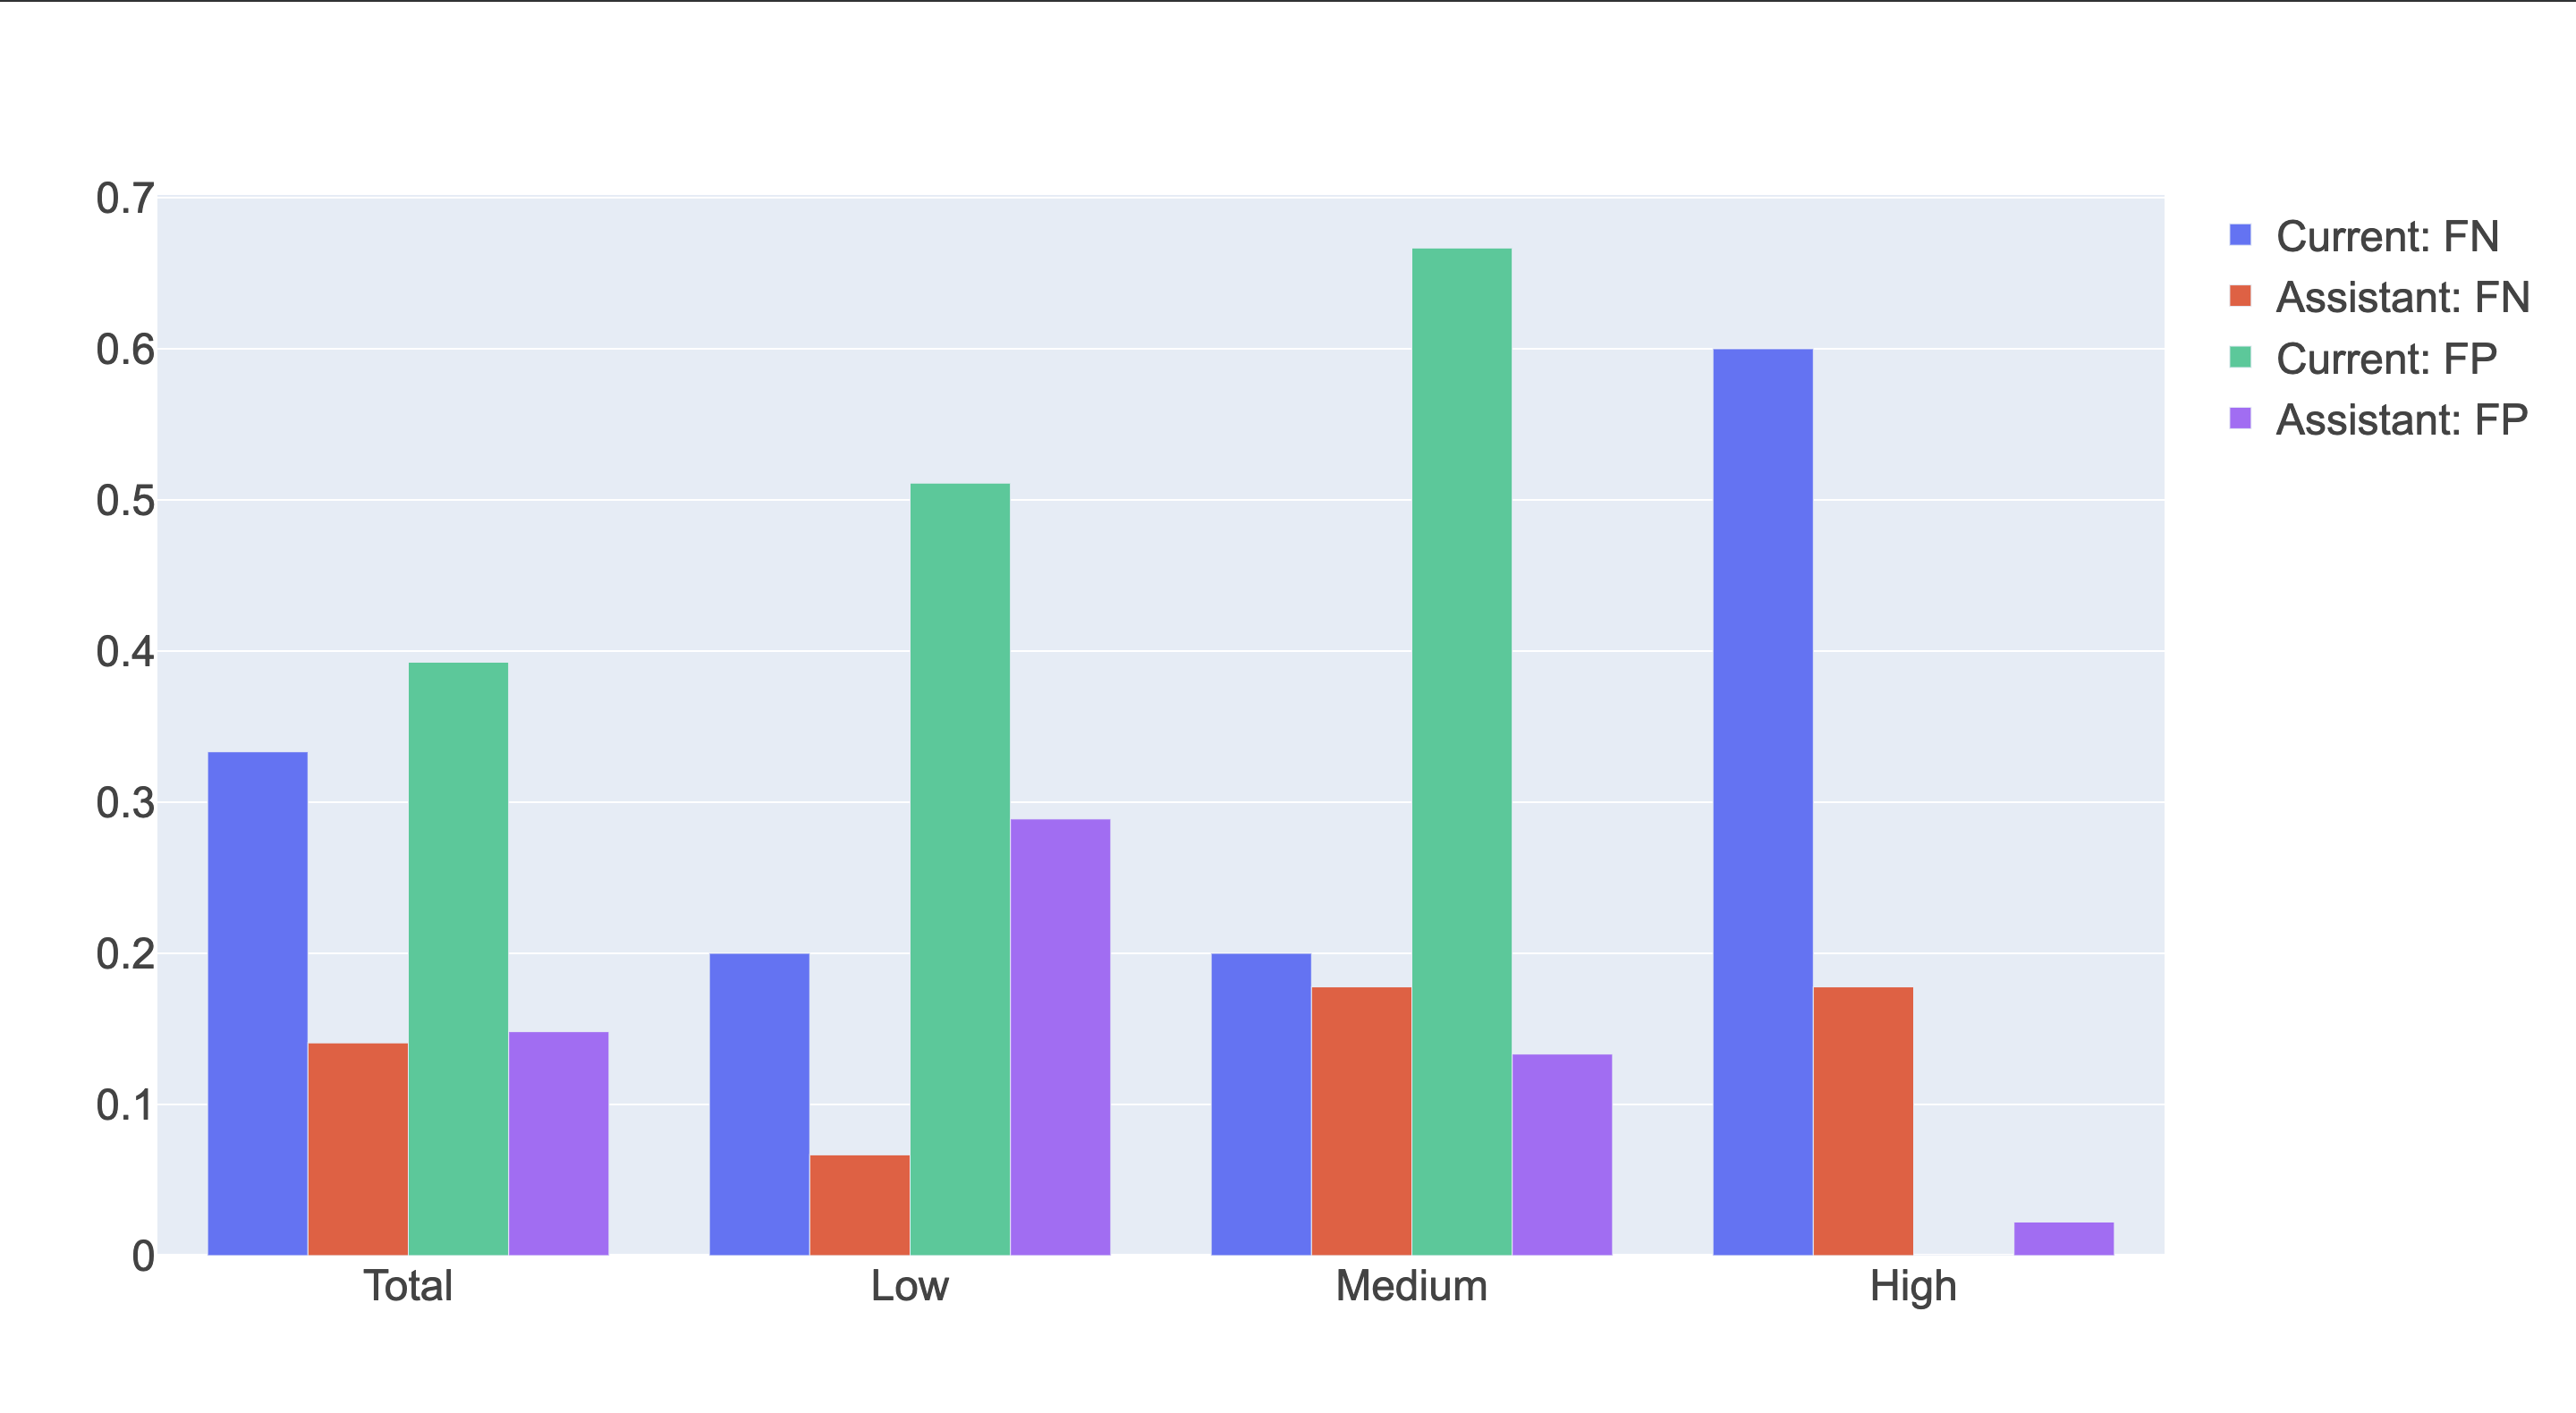
\includegraphics[width=\columnwidth]{images/fig038}
\caption{{\it Current} (Clinician-Only) {\bf vs} {\it Assistant} (Clinician-AI) rates for FNs and FPs. An FN is considered when the BIRADS\textsubscript{provided} $<$ BIRADS\textsubscript{real}. An FP is considered when the BIRADS\textsubscript{provided} $>$ BIRADS\textsubscript{real}.}
\label{fig:fig038}
\end{figure}
%%%%%%%%%%%%%%%%%%%%%%%%%%%%%%%%%%%%%%%%%%%%%%%%%%%

Notably, the introduction of the assistant led to a significant reduction in \ac{FP} rates (Figure~\ref{fig:fig038}), decreasing from 39\% on the {\it current} (Clinician-Only) scenario to 15\% on the {\it assistant} (Clinician-AI) scenario for an overall ({\it i.e.}, Total) condition.
In essence, the intelligent agent will have a 24\% decrease in situations where clinicians are providing a \ac{BI-RADS} higher than the real one.
These findings highlight the effectiveness of the intelligent agent in minimizing false positives and improving diagnostic accuracy.

\subsubsection{Precision \& Recall}
\label{sec:app003004009002}

A correlation exists between groups and accuracy scores.
This is interesting, since the {\it Clinician-AI} (Table~\ref{tab:tab007002}) scenario complies with what we observe for the {\it Clinician-Only} (Table~\ref{tab:tab007001}).
Specifically, it is easier for the clinician to classify exams with {\it Low} and {\it High} severities.
For these cases, higher scores were obtained for both precision and recall.
This contrasts with the classification performance in the exams that belong to {\it Medium} severity.
Table~\ref{tab:tab007001} demonstrates the minimum precision value ($M\textsubscript{Precision} = 0.17$, $SD\textsubscript{Precision} = 0.05$) obtained for the {\it Medium} severity, highlighting the challenges in classifying such cases.
The classification is easier in border scenarios ({\it i.e.}, {\it Low} and {\it High}) compared to the {\it Medium} scenario.
In {\it Low} severity, the typical decision is to assign a pathology of ``no findings'' (no lesion is present), while in {\it High} severity the lesion is often large and exhibits visible (irregular shaped) contours.
However, classification of lesions in the {\it Medium} severity is challenging due to the difficulty in determining whether they are benign or malignant, despite their presence.

%%%%%%%%%%%%%%%%%%%%%%%%%%%%%%%%%%%%%%%%%%%%%%%%%%%
\begin{table}[htbp]
\begin{minipage}{0.45\linewidth}
\centering
\begin{tabular}{ c c c c c c c }
\toprule
\small
&
\multicolumn{2}{ c }{Precision}
&
\multicolumn{2}{ c }{Recall}
\\
\cmidrule(lr){2-3}
\cmidrule(lr){4-5}
\cmidrule(lr){6-7}
Severity & Mean & SD & Mean & SD \\
\bottomrule
Low    & 0.50 & 0.35 & 0.63 & 0.09 \\
Medium & 0.17 & 0.05 & 0.71 & 0.05 \\
High   & 0.60 & 0.02 & 0.59 & 0.14 \\
\bottomrule
\end{tabular}
\caption{The {\it Precision} and {\it Recall} measurements for the {\it Clinician-Only} setup. In this case, we grouped severities into {\it Low}, {\it Medium} and {\it High}.}
\label{tab:tab007001}
\end{minipage}
\hfill
\begin{minipage}{0.45\linewidth}
\centering
\begin{tabular}{ c c c c c c c }
\toprule
\small
&
\multicolumn{2}{ c }{Precision}
&
\multicolumn{2}{ c }{Recall}
\\
\cmidrule(lr){2-3}
\cmidrule(lr){4-5}
\cmidrule(lr){6-7}
Severity & Mean & SD & Mean & SD \\
\bottomrule
Low    & 0.59 & 0.07 & 0.70 & 0.14 \\
Medium & 0.68 & 0.06 & 0.56 & 0.01 \\
High   & 0.96 & 0.12 & 0.77 & 0.25 \\
\bottomrule
\end{tabular}
\caption{The {\it Precision} and {\it Recall} measurements for the {\it Clinician-AI} setup. In this case, we grouped severities into {\it Low}, {\it Medium} and {\it High}.}
\label{tab:tab007002}
\end{minipage}
\end{table}
%%%%%%%%%%%%%%%%%%%%%%%%%%%%%%%%%%%%%%%%%%%%%%%%%%%

The great advantage of the proposed assistant, is that the assistant was able to improve the accuracy of the clinician in the most challenging cases ({\it i.e.}, {\it Medium} severity) where it is hard to perform a reliable and trivial classification.
This can be seen in the proposed {\it Clinician-AI} scenario (Table~\ref{tab:tab007002}), where now a higher score was obtained for the precision ($M\textsubscript{Precision} = 0.68$, $SD\textsubscript{Precision} = 0.06$).
Also note that both {\it Low} and {\it High} severities present superior performance, where the latter exhibits the most notable improvement.

\subsubsection{Accuracy \& Acceptance}
\label{sec:app003004009003}

Now, regarding the qualitative results, the most crucial clinician's opinions and feedback were addressed.
The feedback and results enable us to conclude that this system achieves significantly higher accuracy expectations.
Hence, with the collaboration of clinicians, the assistant will likely improve the rates of \acp{TP} (Figure \ref{fig:fig043}).
In line with these promising results, the level of benevolence was increased, while providing clinicians the opportunity to control the acceptance or rejection of the results.
Nevertheless, the system leads clinicians to higher rates of trust and satisfaction by also providing an assistant as a second opinion.
This study shows that threefold questions:
(1) {\bf Understanding};
(2) {\bf Capability}; and
(3) {\bf Benevolence};
can positively answer this respective requirement.
Also, the existence of {\it heatmaps} was pointed out by 82\% of the clinicians as an essential functionality, promoting higher levels of trust, accuracy, and acceptance of the assistant on the clinical workflow.

\section{Further Reflections}
\label{sec:app003005}

In this work, insights were provided into feasible preparation techniques for clinical end-users interacting with medical decision-making systems for breast cancer diagnosis purposes (Section~\ref{sec:app001006} of Appendix~\ref{chap:app001}).
This is especially valuable as assistant techniques are simple and easy to apply.
As a matter of fact, the {\it BreastScreening-AI} framework is a web-based tool (Section~\ref{sec:app001008} of Appendix~\ref{chap:app001}).
Therefore, it can be deployed on any remote server and accessed via a web browser.
Which is typically available on any computer device.

Before discussing the obtained results for diagnostic precision and recall, the condition's prevalence must first be known.
Specifically, the condition's prevalence is defined as the population percentage that has the condition~\cite{CALISTO2021102607}.
Based on literature~\cite{CALISTO2022102285}, the estimated prevalence of breast cancer is between 0.75 and 0.90 sensitivity and 0.90 to 0.95 specificity.
For this appendix and to better detail what we discussed in Section~\ref{sec:chap005007} of Chapter~\ref{chap:chap005}, a prevalence assumption of the higher end will be made, with a sensitivity of 0.90 and a specificity of 0.95.

Sensitivity is the accuracy of the test on women who have breast cancer.
In other words, if a woman with breast cancer gets imaging reports, the test will come back positive 90\% of the time because the test has a 0.9 sensitivity.
For 10\% of the women with breast cancer, the imaging results will be a \ac{FN}, where the test misdiagnoses a woman who has the disease.
Under this work, the sensitivity of breast cancer was calculated by a combination of radiologist-assessed \ac{BI-RADS} values and Clinician/\ac{AI}-assessed {\it acceptance} or {\it rejection} of the proposed values.
Specificity is the accuracy of the diagnosis for women who do not have breast cancer.
That is, if a woman does not have breast cancer, the test will be negative 95\% of the time.
The other 5\% of the time, the woman gets a \ac{FP}, which means the test is positive for a woman who does not have breast cancer.

Through a user-centered evaluation and analysis~\cite{CALISTO2021102607}, clinicians spent about 89 seconds/image for the {\bf P1} - Low severity, while using the assistant.
On the contrary, clinicians spent about 146 seconds/image, while using a system without any \ac{AI} technique.
Meaning that clinicians have 60\% more of higher time performance with the assistant, in comparison to a system with no \ac{AI}.
Furthermore, by looking at the time spent on the {\bf P2} - Medium severity, clinicians spent almost the same time.
With this assistant, the time spent was 77 seconds/image {\it vs.} 78 seconds/image with no \ac{AI}.
Last but not least, for the {\bf P3} - High severity, clinicians did a 116 seconds/image without \ac{AI} techniques, and with the assistant, clinicians did a 64 seconds/image.

Higher results for {\it Low} and {\it High} severities are affected by several factors.
In {\it Low} severity ({\it i.e.}, no lesion found), even if the radiologist does not see any suspicious region, the clinician wants to make sure about this decision.
In {\it High} ({\it i.e.}, presence of malign lesion), the clinician tends to spend more time to ascertain if there are more lesions to take in consideration.
This means that, for an overall of severity conditions, clinicians are performing with better values of time while interacting with the assistant.
On one hand, the assistant achieve, as well as report, better results of {\it Precision} and {\it Recall} accuracy.
On the other hand, the assistant significantly improves time, accuracy, and acceptance.

Consistent with previous results~\cite{topol2019high}, perceptions and perceived \ac{UX} of clinicians in accepting a novel clinical system are affected by being optimized for high {\it precision} or for higher {\it recall} values.
Taking the {\it Medium} severity as an example (Table~\ref{tab:tab001} and Table~\ref{tab:tab002}), it was observed that 83\% of clinicians made at least one in three patient mistakes, from which 71\% are making higher \acp{FP}.
This aspect underlines the need for more studies regarding {\it Precision/Recall} understanding impact on the workflow.

More granular \ac{ML} annotating tools can be valuable to match the above requirement  on clinical institutions~\cite{Kocielnik:2019:YAI:3290605.3300641}.
By measuring satisfaction, preferences, \ac{FP}/\ac{FN} rates, and time performance, we could conclude that expectation adjustments, such as explicitly explaining the details on what the system can or can not do, will successfully impact the intended aspects of beliefs.
Finally, our results show that these expectation adjustments successfully reduced inter-variability and intra-variability with \ac{AI} assistance.
However, we could observe behavioral differences in decision-making between groups of clinicians.
Leading us to investigate further those differences in Chapter~\ref{chap:chap006}.

In this work, the results show that clinicians' accuracy and acceptance can be improved by introducing an intelligent agent.
Not only in terms of deception, but also in terms of the involved understanding of what the system can do.
Which is used in typical intelligible \ac{AI} works~\cite{10.1145/3173574.3174156}, and can be applied to this type of medical decision-making system.
Ultimately, this addresses an important gap in existing research on preparing clinicians for \ac{AI}-assisted systems.

\subsection{Discussing Clinical Impact}
\label{sec:app003005001}

Expectation adjustments were found to offer a significant improvement in accuracy and acceptance across higher levels of {\it recall}.
Moreover, those adjustments proved practical high {\it precision} and {\it recall} characteristics in which clinicians experienced higher degrees of trust.
It is believed that expectation adjustments are intended for clinicians, but their success depends on the informing capacity of the \ac{DL} models to be aware of their limitations.
For instance, each model should acknowledge its generalizability power for specific cases, such as an imbalanced dataset (Section~\ref{sec:app003004006}).

Although a system fostering higher levels of {\it recall} could increase overall clinicians' expectations, there are cases where high {\it precision} can be considered.
This is especially true for cases with high rates of \acp{FP} and almost nonexistent \acp{FN} paired with the elevated generalizability power of the model for those cases.
An example of that is training a \ac{DL} model with a large dataset of `no findings' (\ac{BI-RADS} = 1) patient cases.
Of course, we are assuming a multi-\acs{DL} model strategy, having several \ac{DL} models with a different focus on precision and recall, as we did between the DenseNet (Section~\ref{sec:app004001001}) and the HyperDenseNet (Section~\ref{sec:app004001002}) for Chapter~\ref{chap:chap006}.
Therefore, adjusting the clinician's expectations depending on the \ac{DL} model characteristics and its limitations for specific tasks is of chief importance.

As explained in this work, a study to expose clinicians to the proposed \ac{AI}-assisted techniques was developed in order to check if the preparation through expectation adjustments can be an effective approach on the clinical domain.
In terms of user expectations, few studies have been performed to evaluate how a \ac{CDSSe} can be implemented in a manner that maximizes their clinical impact.
Even with the presented limitations, it is expected that \ac{HAII} will play a major role in the evaluation of these systems.
In the {\it BreastScreening-AI}, by having a high specificity method to minimize the \ac{FP} outcomes may lead to unnecessary anxiety among patients and negatively impact to the cost-effectiveness.

As we presented in our additional findings (Section~\ref{sec:app003004}), the analysis of significance for high-severity cases (BIRADS $>$ 3) shows that our assistant will impact radiologists' choice of malignant lesions.
The results proved a 51\% accuracy improvement of these high severity cases using our \ac{AI}-assisted system.
With these achieved improvements, it is trivial to understand that \ac{AI} will positively impact the clinical domain.
In short, \ac{AI} is progressively having a cognitive impact in medical practice by applying several AI-assisted techniques ({\it i.e.}, DenseNet~\cite{GOTTAPU2018179}) to rapidly and automatically read the medical images.
As described above, \ac{AI} can provide new paths to optimize healthcare using augmented medical imaging analysis, and may provide new therapies, reducing medical errors and clinical outcomes.

\subsection{Perception Differences}
\label{sec:app003005002}

Directly from medical data, \ac{AI} can advert clinical errors due to cognitive biases, positively impacting patient care.
In this study, the achieved results are showing that, despite several achieved tasks in which the \ac{AI} functionalities are supposed to assist, clinicians should circumspect result decisions for the impact of various types on assistant flaws.
Particularly, a number of aspects should be considered, such as {\it workload}, {\it usability} and {\it usefulness}.

\textcolor{revised}{We measured both {\it mental} and {\it physical} demands, with our \ac{AI} assistant reducing the {\it workload} by 47.78\% (Section~\ref{sec:chap005006001} and Section~\ref{sec:chap005006004} of Chapter~\ref{chap:chap005}).
The {\it mental} measurements shed light on how clinicians perceive the system, especially when dealing with erroneous suggestions and evaluating multiple recommendations.
The {\it physical} measurements provided insights into clinicians' experiences when manually executing new tasks or correcting assistant actions.}
In this study, the document focuses on the {\it Precision} and {\it Recall} problem, since the thesis wants to measure the perception differences of a decision-making system for medical purposes.
Although we summarized the {\it workload} results in Section~\ref{sec:chap005006001} of Chapter~\ref{chap:chap005}, they are detailed and further discussed in this appendix.

To measure {\it workload}, the well known \ac{NASA-TLX} scale was used.
For the statistical significance, the \ac{ANOVA} statistical tests were used in this thesis.
Briefly, both {\it mental} and {\it physical} measurements perceived lower (which is better) with our assistant (F = 2.85) in comparison to the condition without the \ac{AI} technique (F = 7.86).
Both results showed to have a significant impact (p $<$ 0.05) for the two ({\it i.e.}, {\it mental} and {\it physical}) {\it workload} measurements.

For {\it usability}, it was measured in terms of performance and learnability, as well as satisfaction.
Performance denotes the accuracy and completeness of clinicians in accomplishing the specified system functionalities.
Learnability is one of the measurements for effectiveness, and it assists with abilities in functioning the system.
Satisfaction indicates the insights and opinions of the system.
To measure {\it usability}, the well known \ac{SUS} was used.
In short, 86\% of the clinicians agree that the introduction of an intelligent agent will not bring more complexity to the diagnosis task.
Moreover, 85\% of the clinicians preferred the \ac{AI} condition.
Meaning that the overall {\it usability} results are positive.

Finally, {\it usefulness} was also measured in this work.
An early qualitative analysis showed that (41/45) clinicians accept the introduction of an \ac{AI} algorithm to their daily work.
In fact, many of the clinicians said that: ``I would like to frequently use your system on my daily practice'' (C1).
Which is representative for the acceptance of the system.

To conclude this section, with \ac{AI} it is possible to advert clinical errors by taking advantage of the acquired and curated medical data.
At a same time, not only patient care was improved, but also several other aspects for clinicians.
From accuracy of the diagnostic results, to the reduction of clinicians' {\it workload}.
With the introduction of the proposed \ac{AI}-assisted techniques, several perception differences of the cognitive biases so present on the medical decision-making systems were improved.

\subsection{Observed Outcomes}
\label{sec:app003005003}

The output classification (present information) of this network always depend on the images that the network received previously (past information).
While this is only one class of \ac{CDSSe}, we believe this class of systems represents many current efforts of integrating \ac{HAII} into other clinical domains ({\it e.g.}, systems for clinical drug development, epidemiology, dementia treatment)~\cite{Savage2019, shah2019artificial, topol2019high}.

In critical systems, it is more important to analyze the severity of the consequences.
However, the severity of consequences applies to different clinical decision-making ({\it i.e.}, the classification) doubts rather than any medical imaging workload improvements ({\it e.g.}, drug development, epidemiology, or dementia treatment).
For instance, one of the major doubts and difficulties came from the {\it Medium} cases, which must be a higher concern regarding explanations.
To accomplish this, when the clinician presses the {\it Explain} button, the information showed by the {\it heatmaps} must further cover those cases.

When comparing the clinicians' behavior with respect to {\it Clinician-Only} vs. {\it Clinician-AI}, system requirements were obtained, which encompass the current practices and the future of \ac{AI}-assisted diagnosis.
One important requirement was to provide clinician control over the proposed \ac{BI-RADS} resulting from the \ac{AI} algorithm.
With the {\it Accept} and {\it Reject} buttons, the clinician can control the final diagnostic value.
In the case of {\it Reject}, the clinician can even input and provide the new \ac{BI-RADS} value.

The importance of avoiding the different types of errors depends on the information available from a specific clinical domain.
While the thesis could argue that in breast cancer diagnosis, \acp{FN} are always better to avoid, the solution can not always suggest independently regarding the clinical domain.
In the breast cancer domain, missing \acp{FP} has more impact on the patient's condition, than marking an \ac{FP}.

From other clinical domains, an \ac{FP} might be more important to avoid.
For instance, on drug development, the field wants to prefer avoiding the \ac{FP} rates.
By doing that, the field is optimizing the number of chemicals and drugs identified incorrectly by the system~\cite{raja2017machine}.
Having that said, it is believed that these findings are generalizing a solution to a clinical class of passive systems ({\it i.e.}, clinicians are making the final decisions) in which the end ratio of workload regarding both \acp{FP} and \acp{FN} is lower.

\subsection{Further Work}
\label{sec:app003005004}

Breast cancer screening is one of the nuclear topics in medical imaging analysis.
Under this thesis, it is believed that with the proposed assistant, intelligent agents are able to change diagnosis paradigm.
Results are indicating that it is possible to introduce behavioral change on the clinical workflow in a \ac{HAII} manner.
Further work will include other deep network architectures, besides the DenseNet used herein and to generate attention maps as an alternative to the heatmaps.
That is, it will include not only the classification output (as proposed in this thesis) but also, the segmentation map of the lesion.
This will be done automatically and integrated in the \ac{UI}.

Other interesting future work is related with the data used. 
In this chapter, the study was performed with a dataset of images from one institution.
Could be interesting to enlarge the clinician number from this institution, and also enlarging the data from other institutions.
This is interesting, since in recent years, many \ac{ML} models have been proposed to accurately diagnose breast cancer.
However, when these models are tested on unseen datasets, acquired with different devices and scanners, their performance is usually reduced.
Thus, there exist a need to build generalizable models that can be applied consistently across clinical institutions.

\section{Final Remarks}
\label{sec:app003006}

In this appendix, it was developed and studied {\it BreastScreening-AI}, an \ac{AI}-assisted clinical imaging support system which provides an automated diagnosis based on \ac{DL} methods.
The study deployed and tested {\it BreastScreening-AI} in a real-world scenario with 45 clinicians from nine clinical institutions to experiment with several techniques of \acp{HAII}.
Results show improvements in clinician’s accuracy, as well as acceptance of an \ac{AI}-assisted system on the clinical domain for the breast cancer diagnosis.
Also, results are showing that by focusing on both {\it Precision} and {\it Recall} problem, the higher rates of the system will perform at the same level of accuracy, leading to much higher perceptions of accuracy.
Hence, increasing acceptance of the system by the medical professionals.

Before \ac{AI}-assisted techniques can be used in medicine, it is first a need to go through clinical trials, so that the final solution can establish the system validity.
It is vital to make sure that the model actually provides benefit and guarantee the value to clinicians, as well as to the final patient.
Advances in precision medicine will bring more diagnostic tests and information with more treatment options.
Which will only increase the workload of clinicians and decrease of expectations.
Indeed, the introduction of \ac{AI} systems in the clinical workflow will change medical interventions.
The findings open the way of shaping expectations among medical decision-making as an effective way of improving clinician’s acceptance of \ac{AI} systems on the clinical domain.